\documentclass{amsart}

%%%%%%%%%%%%%%%%%%%%%%%%%%%%%%%%%%%%%%%%%%%%%%%%%%%%%%%%%%%%%%%%
%  packages
%   
%%%%%%%%%%%%%%%%%%%%%%%%%%%%%%%%%%%%%%%%%%%%%%%%%%%%%%%%%%%%%%%%
\usepackage[all]{xy}     % xmatrix 
\usepackage{graphicx}    % EPS 
\usepackage{bm}          
\usepackage{amsthm}
\usepackage{amsfonts}
\usepackage{latexsym}
\usepackage{amsmath}
\usepackage{amssymb}
\usepackage{graphicx}
\usepackage{float}



%%%%%%%%%%%%%%%%%%%%%%%%%%%%%%%%%%%%%%%%%%%%%%%%%%%%%%%%%%%%%%%%
%  ×Ô¶¨ÒåÃüÁî
%%%%%%%%%%%%%%%%%%%%%%%%%%%%%%%%%%%%%%%%%%%%%%%%%%%%%%%%%%%%%%%%
\newcommand{\A}{\mathcal A}
\newcommand{\AAA}{\mathfrak A}
\newcommand{\B}{\mathcal B}
\newcommand{\BBB}{\mathfrak B}
\newcommand{\CCC}{\mathcal C}
\newcommand{\DDD}{\mathcal D}
\newcommand{\F}{\mathcal F}
\newcommand{\G}{\mathcal G}
\newcommand{\HHH}{\mathcal H} %for Hilbert space
\newcommand{\LLL}{\mathcal L} % for lattice
\newcommand{\PPP}{\mathcal P}
\newcommand{\M}{\mathcal M}
\newcommand{\MMM}{\mathfrak M}
\newcommand{\NNN}{\mathcal N} %for nest
\newcommand{\RRR}{\mathcal R}
\newcommand{\SSS}{\mathcal S}
\newcommand{\W}{\mathcal W}
\newcommand{\ZZZ}{\mathcal Z}
\newcommand{\supp}{\mathop{\mathrm supp}}
\newcommand{\TT}{\mathcal T}
\newcommand{\II}{\mathrm{II}}


\newcommand{\e}[2][]{e^{#1}_{#2}} %for matrix unit \e[upper index]{lower index}

\newcommand{\Lat}{\mathrm{Lat}}
\newcommand{\Alg}{\mathrm{Alg}}
\newcommand{\tensor}{\mathop{\bar \otimes}}
\newcommand{\tr}{\tau}

\newcommand{\C}{\mathbb C} %for complex numbers
\newcommand{\R}{\mathbb R}  %for real numbers
\newcommand{\Z}{\mathbb Z} %for integers
\newcommand{\N}{\mathbb N} % for natural numbers

\newtheorem{theorem}{Theorem}[section]
\newtheorem{corollary}{Corollary}[section]
\newtheorem{main}{Main Theorem}[section]
\newtheorem{lemma}{Lemma}[section]
\newtheorem{prop}{Proposition}[section]
\newtheorem{df}{Definition}[section]
\newtheorem{remark}{Remark}[section]
\newtheorem{example}{Example}[section]
\newtheorem{question}{Question}[section]


%%%%%%%%%%%%%%%%%%%%%%%%%%%%%%%%%%%%%%%%%%%%%%%%%%%%%%%%%%%%%%%%
%  ¶¨Òå±êÌâ¸ñʽ£¬°üÀ¨title£¬author£¬affiliation£¬emailµÈ¡£
%%%%%%%%%%%%%%%%%%%%%%%%%%%%%%%%%%%%%%%%%%%%%%%%%%%%%%%%%%%%%%%%
\title{Sphere}
%\author{}
%\address{Your address}
%\email{yuanwei.cn@gmail.com}
%\thanks{Research supported by the NSF }
%\keywords{your keywords}
\date{}

\begin{document}

\section{Isomorphism fix the sphere}
Let
\begin{align*}
Q_{\infty}&= \left(
        \begin{array}{cc}
          I & 0 \\
          0 & 0 \\
        \end{array}
      \right),
Q_{0} = \left(
          \begin{array}{cc}
            H_{1} & \sqrt{H_{1}(I-H_{1})} \\
            \sqrt{H_{1}(I-H_{1})} & I-H_{1} \\
          \end{array}
        \right) , \\
Q_{-1}&= \left(
          \begin{array}{cc}
            H_{2} & \sqrt{H_{2}(I-H_{2})}V \\
            V^{*}\sqrt{H_{2}(I-H_{2})} & V^{*}(I-H_{2})V \\
          \end{array}
        \right) \mbox{.}
\end{align*}
be three free projections. Let $\F_3$ be the lattice generated by $\{Q_{\infty}$, $Q_{0}$, $Q_{-1} \}$,
and $\M \otimes M_2(\C) = \F_3''$, the von Neumann algebra generated by $\F_3$.
In \cite{GYII}, we have the following result:

\begin{theorem}
For any projection $Q$
in $\Lat(\Alg(\F_3)) \setminus \{0, I, Q_{\infty}\}$, there are $K_{z}$ and
$U_{z}$ in $\M$ such that
\begin{align*}
Q = Q_{z} = \left(
     \begin{array}{cc}
      K_{z} & \sqrt{K_{z}(I-K_{z})}U_{z} \\
      U_{z}^{*}\sqrt{K_{z}(I-K_{z})} & U_{z}^{*}(I-K_{z})U_{z} \\
  \end{array}
\right) ,
\end{align*}
where
\begin{equation}\label{(*)}
\begin{split}
\sqrt{K_{z}(I-K_{z})^{-1}}U_{z} = &(1+z)\sqrt{H_{1}(I-H_{1})^{-1}}-
                                   z\sqrt{H_{2}(I-H_{2})^{-1}}V \\
                                 &=zS + \sqrt{H_{1}(I-H_{1})^{-1}},
\end{split}
\end{equation}
and $S = \sqrt{H_{1}(I-H_{1})^{-1}}- \sqrt{H_{2}(I-H_{2})^{-1}}V$
for some $z \in \C$. Moreover for any given
$z$ in $\C$, the polar decomposition determines $U_z$ and $K_z$
uniquely which give rise to a projection $Q_z$ (in the above form)
in $\Lat(\Alg(\F_3))$.
\end{theorem}

In another word, by fixing $Q_{\infty}$, we give a coordinate chart of $\Lat\Alg(\F_3) \setminus
\{0, I, Q_{\infty} \}$.

\begin{lemma}
Let $\LLL$ and $\widetilde{\LLL}$ be two reflexive lattices, $\AAA = \LLL''$ and $\widetilde{\AAA} = \widetilde{\LLL}''$.  If $\{ P_{i} \}_{i \in I}$ and
$\{ Q_{i} \}_{i \in I}$ are in $\LLL$ and $\widetilde{\LLL}$ respectively,
and $\Lat(\Alg(\{ P_{i} \}_{i \in I})) = \LLL$, $\Lat(\Alg(\{ Q_{i} \}_{i \in I})) = \widetilde{\LLL}$. Let $\varphi \in Aut(\AAA)$, if $\varphi(\{ P_{i} \}_{i \in I})
= \{ Q_{i} \}_{i \in I}$, then $\varphi(\LLL) = \widetilde{\LLL}$.
\end{lemma}

\begin{proof}
Since we have already showed that if $\LLL$ is a reflexive lattice, and $\varphi \in Aut(\LLL'')$, then
$\varphi(\LLL)$ is also reflexive. So by the fact that $\varphi(\LLL) \supseteq \varphi(\{ P_{i} \}_{i \in I})
= \{ Q_{i} \}_{i \in I}$, it is not hard to see
\begin{align*}
\varphi(\LLL) \supseteq \Lat(\Alg(\{ Q_{i} \}_{i \in I})) = \widetilde{\LLL}.
\end{align*}
By considering $\varphi^{-1}$, we also have
\begin{align*}
\varphi^{-1}(\widetilde{\LLL}) \supseteq \LLL,
\end{align*}
which implies $\widetilde{\LLL} \supseteq \varphi(\LLL)$, thus $\widetilde{\LLL} = \varphi(\LLL)$.
\end{proof}

By the symmetry of the three free projections $Q_{\infty}$, $Q_{0}$, $Q_{-1}$,
any permutation of $\{Q_{\infty}, Q_{0}, Q_{-1} \}$ will give a new coordinate chart of $\LLL = \Lat\Alg(\F_3) \setminus
\{0, I \}$. In another word, if $\varphi \in Aut(\LLL'')$ such that $\varphi(\{Q_{\infty}, Q_{0}, Q_{-1} \})
= \{Q_{\infty}, Q_{0}, Q_{-1} \}$, then by the above lemma, there exists $f: \C \cup \{\infty \} \rightarrow \C \cup \{\infty \}$
such that
\begin{align*}
\varphi(Q_{z}) = Q_{f(z)}.
\end{align*}

For the rest of this note, we will show what this $f$ is. Before that, we first rewrite the equation (1) as following:

\begin{equation}\label{(*)}
\begin{split}
&(1+z)(I - Q_{\infty}Q_{0}Q_{\infty})^{-1}[Q_{\infty}Q_{0}(I-Q_{\infty})] \\
& - z(I - Q_{\infty}Q_{-1}Q_{\infty})^{-1}[Q_{\infty}Q_{-1}(I-Q_{\infty})] \\
&= (I - Q_{\infty}Q_{z}Q_{\infty})^{-1}[Q_{\infty}Q_{z}(I-Q_{\infty})].
\end{split}
\end{equation}

\begin{lemma}
With the notations above, if $\varphi(Q_{\infty}) = Q_{\infty}$, $\varphi(Q_{0}) = Q_{-1}$,
and $\varphi(Q_{-1}) = Q_{0}$, then $f(z) = -1 - z$.
\end{lemma}

\begin{proof}
By applying $\varphi$ on both sides of (2), and the definition of $f$ we have
\begin{equation}\label{(*)}
\begin{split}
&(1+z)(I - Q_{\infty}Q_{-1}Q_{\infty})^{-1}[Q_{\infty}Q_{-1}(I-Q_{\infty})] \\
& - z(I - Q_{\infty}Q_{0}Q_{\infty})^{-1}[Q_{\infty}Q_{0}(I-Q_{\infty})] \\
&= (I - Q_{\infty}Q_{f(z)}Q_{\infty})^{-1}[Q_{\infty}Q_{f(z)}(I-Q_{\infty})].
\end{split}
\end{equation}
Compare (2), (3), we have $f(z) = -1 - z$.
\end{proof}

Now if we consider $\varphi \in Aut(\LLL'')$ such that $\varphi(Q_{-1}) = Q_{-1}$,
$\varphi(Q_{\infty}) = Q_{0}$, $\varphi(Q_{0}) = Q_{\infty}$, we know that
\begin{align}
f(-1) = -1, \qquad f(0) = \infty, \qquad f(\infty) = 0.
\end{align}
By the results above, we will expect that $f$ gives a automorphism of the Riemann sphere, thus
is a $M\ddot{o}bius$ transform, and the only $M\ddot{o}bius$ transforms satisfies (4) is $f(z) = \frac{1}{z}$.
Next we will show that this is indeed the case.

\begin{lemma}
With the notations above, if $\varphi \in Aut(\LLL'')$ such that $\varphi(Q_{-1}) = Q_{-1}$,
$\varphi(Q_{\infty}) = Q_{0}$, $\varphi(Q_{0}) = Q_{\infty}$, then $f(z) = \frac{1}{z}$.
\end{lemma}

\begin{proof}
Again by applying $\varphi$ on the both side of (2), we have
\begin{equation}\label{(*)}
\begin{split}
&(1+z)(I - Q_{0}Q_{\infty}Q_{0})^{-1}[Q_{0}Q_{\infty}(I-Q_{0})] \\
& - z(I - Q_{0}Q_{-1}Q_{0})^{-1}[Q_{0}Q_{-1}(I-Q_{0})] \\
&= (I - Q_{0}Q_{f(z)}Q_{0})^{-1}[Q_{0}Q_{f(z)}(I-Q_{0})].
\end{split}
\end{equation}
Let $W = \left(
           \begin{array}{cc}
             \sqrt{H_1} & \sqrt{I-H_1} \\
             \sqrt{I-H_1} & -\sqrt{H_1} \\
           \end{array}
         \right)$($\in \LLL''$), $WQ_{0}W = Q_{\infty}$ and $WQ_{\infty}W = Q_{0}$. Thus
\begin{equation}\label{(*)}
\begin{split}
&(1+z)(I - Q_{\infty}Q_{0}Q_{\infty})^{-1}[Q_{\infty}Q_{0}(I-Q_{\infty})] \\
& - z(I - Q_{\infty}WQ_{-1}WQ_{\infty})^{-1}[Q_{\infty}WQ_{-1}W(I-Q_{\infty})] \\
&= (I - Q_{\infty}WQ_{f(z)}WQ_{\infty})^{-1}[Q_{\infty}WQ_{f(z)}W(I-Q_{\infty})].
\end{split}
\end{equation}
Remember that
\begin{align*}
Q_{z} = \left(
     \begin{array}{cc}
      K_{z} & \sqrt{K_{z}(I-K_{z})}U_{z} \\
      U_{z}^{*}\sqrt{K_{z}(I-K_{z})} & U_{z}^{*}(I-K_{z})U_{z} \\
  \end{array}
\right),
\end{align*}
By direct computation we know for any $z \in \C$,
\begin{align*}
(WQ_{z}W)_{1,1} &= \sqrt{H_1}K_{z}\sqrt{H_1} + \sqrt{I - H_1}U^{*}_{z}\sqrt{K_{z} (I - K_{z})}\sqrt{H_1} \\
                & \qquad +\sqrt{H_1}\sqrt{K_{z}(I-K_{z})}U_{z}\sqrt{I-H_1} + \sqrt{I-H_1}U^{*}_{z}(I - K_z)U_{z}\sqrt{I - H_1}.
\end{align*}
So by (2) we have
\begin{align*}
I - (WQ_{z}W)_{1,1} &= \sqrt{H_1}(I - K_{z})\sqrt{H_1} - \sqrt{I - H_1}U^{*}_{z}\sqrt{K_{z} (I - K_{z})}\sqrt{H_1} \\
                    & \qquad \qquad - \sqrt{H_1}\sqrt{K_{z}(I-K_{z})}U_{z}\sqrt{I-H_1} + \sqrt{I-H_1}U^{*}_{z}K_{z}U_{z}\sqrt{I - H_1}\\
                    &= \sqrt{H_1}(I-K_z)(\sqrt{\frac{H_1}{I-H_1}} - \sqrt{\frac{K_z}{I - K_z}}U_z)\sqrt{I-H_1} \\
                    & \qquad \qquad- \sqrt{I-H_1}U_{z}^{*}\sqrt{K_{z}(I- K_z)}(\sqrt{\frac{H_1}{I-H_1}} - \sqrt{\frac{K_z}{I - K_z}}U_z)\sqrt{I-H_1}\\
                    & = -z[\sqrt{H_1}(I-K_z)-\sqrt{I - H_1}U^{*}_{z}\sqrt{K_{z}(I-K_z)}]S\sqrt{I-H_1}\\
                    &= -z\sqrt{I-H_1}(\sqrt{\frac{H_1}{I-H_1}} - U^{*}_{z}\sqrt{\frac{K_z}{I-K_z}})(I-K_z)S\sqrt{I-H_1}\\
                    &= |z|^{2}\sqrt{I-H_1}S^{*}(I-K_z)S\sqrt{I-H_1}.
\end{align*}
Similarly, direct computation and (2) will give
\begin{align*}
(WQ_{z}W)_{1,2} &= \sqrt{H_1}K_{z}\sqrt{I - H_1} + \sqrt{I - H_1}U^{*}_{z}\sqrt{K_{z} (I - K_{z})}\sqrt{I - H_1} \\
                & \qquad \qquad -\sqrt{H_1}\sqrt{K_{z}(I-K_{z})}U_{z}\sqrt{H_1} - \sqrt{I-H_1}U^{*}_{z}(I - K_z)U_{z}\sqrt{H_1}\\
                &= -\sqrt{H_1}(I-K_{z})\sqrt{I - H_1} + \sqrt{I - H_1}U^{*}_{z}\sqrt{K_{z} (I - K_{z})}\sqrt{I - H_1} \\
                & \qquad \qquad -\sqrt{H_1}\sqrt{K_{z}(I-K_{z})}U_{z}\sqrt{H_1} + \sqrt{I-H_1}U^{*}_{z}K_{z}U_{z}\sqrt{H_1}\\
                & = \sqrt{I-H_1}(U^{*}_{z}\sqrt{\frac{K_z}{I-K_z}} - \sqrt{\frac{H_1}{I - H_1}})(I-K_z)\sqrt{I - H_1} \\
                & \qquad \qquad + \sqrt{I-H_1}(U^{*}_{z}\sqrt{\frac{K_z}{I-K_z}} - \sqrt{\frac{H_1}{I - H_1}})\sqrt{K_{z}(I-K_z)}U_{z}\sqrt{H_1}\\
                &= \overline{z}\sqrt{I-H_1}S^{*}[(I-K_z)\sqrt{I - H_1} + \sqrt{K_{z}(I-K_z)}U_{z}\sqrt{H_1}]\\
                &= \overline{z}\sqrt{I-H_1}S^{*}(I-K_z)(\sqrt{I-H_1} + \sqrt{\frac{K_z}{I - K_z}}U_{z}\sqrt{H_1})\\
                &= \overline{z}\sqrt{I-H_1}S^{*}(I-K_z)(zS\sqrt{H_1} + \frac{I}{\sqrt{I-H_1}}).
\end{align*}
Thus
\begin{equation}\label{(*)}
\begin{split}
[I - (WQ_{z}W)_{1,1}]^{-1}(WQ_{z}W)_{1,2} &= (\frac{1}{|z|^{2}}\frac{I}{\sqrt{I-H_1}}S^{-1}\frac{I}{I-K_z}{S^{*}}^{-1}\frac{I}{\sqrt{I-H_1}})\\
                                          & \times \overline{z}\sqrt{I-H_1}S^{*}(I-K_z)(zS\sqrt{H_1} + \frac{I}{\sqrt{I-H_1}}) \\
                                          &= \sqrt{\frac{H_1}{I-H_1}} + \frac{1}{z}\frac{1}{\sqrt{I-H_1}}S^{-1}\frac{1}{\sqrt{I-H_1}}.
\end{split}
\end{equation}
Let
\begin{align*}
WQ_{-1}W = \left(
             \begin{array}{cc}
               H_{2}' & \sqrt{H_{2}'(I - H_{2}')}V' \\
               {V'}^{*}\sqrt{H_{2}'(I - H_{2}')} & {V'}^{*}(I - H_{2}') V'  \\
             \end{array}
           \right),
\end{align*}
by (7) we have
\begin{align*}
\sqrt{\frac{H_{2}'}{I - H_{2}'}}V' = \sqrt{\frac{H_1}{I-H_1}} - \frac{1}{\sqrt{I-H_1}}S^{-1}\frac{1}{\sqrt{I-H_1}}.
\end{align*}
So we may rewrite the equation in (7),
\begin{align}
[I - (WQ_{f(z)}W)_{1,1}]^{-1}(WQ_{f(z)}W)_{1,2} = (\frac{1}{f(z)} + 1)\sqrt{\frac{H_1}{I-H_1}} - \frac{1}{f(z)}\sqrt{\frac{H_{2}'}{I - H_{2}'}}V'.
\end{align}
Since $Q_{\infty}$, $Q_{0}$ and $WQ_{-1}W$ are also free, we know that
\begin{align}
[I - (WQ_{f(z)}W)_{1,1}]^{-1}(WQ_{f(z)}W)_{1,2} = (z + 1)\sqrt{\frac{H_1}{I-H_1}} - z \sqrt{\frac{H_{2}'}{I - H_{2}'}}V'.
\end{align}
(This fact can also be deduced from (6)). Compare (8) and (9), we know $f(z) = \frac{1}{z}$.
\end{proof}

Now we introduce some notations.

Let $\varphi_{1} \in Aut(\LLL'')$ be the automorphism such that $\varphi_{1}(Q_{\infty}) = Q_{\infty}$, $\varphi_{1}(Q_{0}) = Q_{-1}$,
and $\varphi_{1}(Q_{-1}) = Q_{0}$, and $f_1$ be the map such that $\varphi_{1}(Q_{z}) = Q_{f_{1}(z)}$, then $f_{1}(z) = -1 -z$.

Let $\varphi_{2} \in Aut(\LLL'')$ be the automorphism such that $\varphi_{2}(Q_{-1}) = Q_{-1}$, $\varphi_{2}(Q_{0}) = Q_{\infty}$,
and $\varphi_{2}(Q_{\infty}) = Q_{0}$, and $f_2$ be the map such that $\varphi_{2}(Q_{z}) = Q_{f_{2}(z)}$, then $f_{2}(z) = \frac{1}{z}$.

\begin{corollary}
Let $\varphi_{3} \in Aut(\LLL'')$ be the automorphism such that $\varphi_{3}(Q_{0}) = Q_{0}$, $\varphi_{3}(Q_{\infty}) = Q_{-1}$,
and $\varphi_{3}(Q_{-1}) = Q_{\infty}$, and $f_3$ be the map such that $\varphi_{3}(Q_{z}) = Q_{f_{3}(z)}$.
Since $\varphi_{3} = \varphi_{1}\circ \varphi_{2} \circ \varphi_{1}$, then $f_{3}(z) = \frac{-z}{z+1}$.
\end{corollary}

\begin{corollary}
Let $\varphi_{4} \in Aut(\LLL'')$ be the automorphism such that $\varphi_{4}(Q_{0}) = Q_{-1}$, $\varphi_{4}(Q_{\infty}) = Q_{0}$,
and $\varphi_{4}(Q_{-1}) = Q_{\infty}$, and $f_4$ be the map such that $\varphi_{4}(Q_{z}) = Q_{f_{4}(z)}$.
then $f_{4}(z) = \frac{-1}{z+1}$.
\end{corollary}

\begin{remark}
The results (except lemma 1) in this note depend on the fact that  $\{Q_{\infty}$, $Q_{0}$, $Q_{-1} \}$ are
free, because otherwise the automorphism which permutes these three projections may not exist.
\end{remark}

Since $\{I - Q_{\infty}, I - Q_{0}, I - Q_{-1} \}$ are three free projections, then the map
\begin{align*}
Q_{\infty} \rightarrow I - Q_{\infty}, \qquad Q_{0} \rightarrow I - Q_{0}, \qquad Q_{-1} \rightarrow I - Q_{-1},
\end{align*}
induce a *-isomorphism of $\LLL''$. Also we know that $\Lat\Alg(\{I - Q_{\infty}, I - Q_{0}, I - Q_{-1} \}) =
\{I - Q | Q \in \LLL \}$.

\begin{lemma}
Let $\varphi$ be the *-isomorphism of $\LLL''$ such that $\varphi(Q_{\infty}) = I - Q_{\infty}$, $\varphi(Q_{0}) = I - Q_{0}$,
$\varphi(Q_{-1}) = I - Q_{-1}$, then  $\varphi(Q_{z}) = I - Q_{\overline{z}}$.
\end{lemma}

\begin{proof}
By the discussion above, we know there exists a function $f : \C \cup \{\infty \} \rightarrow \C \cup \{\infty\}$ such
that $\varphi(Q_{z}) = I - Q_{f(z)}$.
Applying $\varphi$ on both side of the equation (2), we have
\begin{align*}
&(1+z)[I - (I - Q_{\infty})(I - Q_{0})(I - Q_{\infty})]^{-1}[(I - Q_{\infty})(I - Q_{-1})Q_{\infty}] \\
& - z[I - (I-Q_{\infty})(I - Q_{-1})(I - Q_{0})]^{-1}[(I - Q_{\infty})(I - Q_{-1})Q_{\infty}] \\
&= [I - (I - Q_{\infty})(I - Q_{f(z)})(I - Q_{\infty})]^{-1}[(I - Q_{\infty})(I - Q_{f(z)})Q_{\infty}],
\end{align*}
which implies
\begin{align*}
(1+z)\sqrt{H_{1}(I - H_{1})^{-1}} -zV^{*}\sqrt{H_{2}(I - H_{2})^{-1}} = U^{*}_{f(z)}\sqrt{K_{f(z)}(I - K_{f(z)})^{-1}}.
\end{align*}
Thus by (1), we have $f(z) = \overline{z}$.
\end{proof}

\begin{corollary}
$\| Q_{z_1} - Q_{z_2} \|_{2} = \| Q_{\overline{z}_1} - Q_{\overline{z}_2} \|_{2}$.
\end{corollary}

\begin{proof}
By the notations in the above lemma, we have
\begin{align*}
\| Q_{z_1} - Q_{z_2} \|_{2} = \| \varphi(Q_{z_1}) - \varphi(Q_{z_2}) \|_{2} =  \|(I - Q_{\overline{z}_1}) - (I - Q_{\overline{z}_2}) \|_{2}
=  \| Q_{\overline{z}_1} - Q_{\overline{z}_2} \|_{2}.
\end{align*}
\end{proof}

\section{distance formula}

In this section, we will compute the distance between $\parallel Q_{z} - Q_{\infty} \parallel_{2}$.Note that
\begin{align*}
\parallel Q_{z} - Q_{\infty} \parallel_{2}^{2} = 1-2tr(Q_{z}Q_{\infty}) = 1 - \tau(Q_{\infty}Q_{z}Q_{\infty}|_{Q_{\infty}\HHH}),
\end{align*}
where $tr$ is the trace on $\F_{3}''$, and $\tau$ is the trace on $Q_{\infty}\F_{3}''Q_{\infty}$, such that
\begin{align*}
tr(\left(
     \begin{array}{cc}
       A_{11} & A_{12} \\
       A_{21} & A_{22} \\
     \end{array}
   \right)) = \frac{1}{2}(\tau(A_{11}) + \tau(A_{22})).
\end{align*}

Remember that
\begin{align*}
Q_{z} = \left(
     \begin{array}{cc}
      K_{z} & \sqrt{K_{z}(I-K_{z})}U_{z} \\
      U_{z}^{*}\sqrt{K_{z}(I-K_{z})} & U_{z}^{*}(I-K_{z})U_{z} \\
  \end{array}
\right) ,
\end{align*}
where
\begin{align*}
\sqrt{K_{z}(I-K_{z})^{-1}}U_{z} = (1+z)\sqrt{H_{1}(I-H_{1})^{-1}}-
                                   z\sqrt{H_{2}(I-H_{2})^{-1}}V.
\end{align*}
In order to compute $\tau(K_{z})$, we will use the technique developed by Haagerup and Schultz in \cite{HH}.

We first introduce some notations.

Let $\AAA$ be a finite von Neumann algebra with faithful, tracial state $\tau$, we will use $\widetilde{\AAA}$ to denote the set of
closed, densely defined operators affiliated with $\AAA$. Recall that every operator $T \in \widetilde{\AAA}$
has a polar decomposition
\begin{align*}
T = U|T| = U\int^{\infty}_{0} t dE_{|T|}(t),
\end{align*}
where $U \in \AAA$ is a unitary, and the spectral measure $E_{|T|}$ takes values in $\AAA$. In particular,
for $T \in \widetilde{\AAA}$ we may define $\mu_{|T|} \in Prob(\R)$ by
\begin{align*}
\mu_{|T|}(B) = \tau(E_{|T|}(B)),  (B \in \mathbb{B}),
\end{align*}
where $\mathbb(B)$ is set of Borel subset of $\R$.

\begin{df}
For $\mu \in Prob(\R, \mathbb{B})$ let $\widetilde{\mu}$ denote the symmetrization of $\mu$. That
is $\widetilde{\mu} \in Prob(\R, \mathbb{B})$ is given by
\begin{align*}
\widetilde{\mu}(B) = \frac{1}{2}(\mu(B) + \mu(-B)), (B \in \mathbb{B}).
\end{align*}
\end{df}

\begin{prop}[Proposition 3.11 in \cite{HH}]
Let $S$, $T \in \widetilde{\AAA}$ be *-free R-diagonal elements. Then
\begin{align*}
\widetilde{\mu}_{|S+T|} = \widetilde{\mu}_{|S|}\boxplus \widetilde{\mu}_{|T|}.
\end{align*}
\end{prop}

Since we may treat $K_z$ as the summation of two *-free R-diagonal elements, then by
the above proposition, we can compute the distribution of $K_z$.

\begin{lemma}
By the notation above, we have
\begin{align*}
d \mu_{\sqrt{\frac{K_z}{I-K_z}}}(t) = \frac{2}{\pi}\frac{|z|+|z+1|}{t^2 + (|z|+|z+1|)^2} 1_{(0, \infty)}(t) dt .
\end{align*}
\end{lemma}
\begin{proof}
Since the distribution of $H_i$($i = 1$, $2$) has the same distribution as $cos^2\frac{\pi}{2}\theta$ on $[0, 1]$, thus $\sqrt{\frac{H_i}{I - H_i}}$ has
the same distirubtion as $cot\frac{\pi}{2}\theta$ on $[0, 1]$. We have
\begin{align*}
d\mu_{\sqrt{\frac{H_i}{I - H_i}}}(t) = \frac{2}{\pi}\frac{1}{1+t^2} 1_{(0, \infty)} dt.
\end{align*}
Then for any $r \in \R^{+}$,
\begin{align*}
d\mu_r(t) = d\mu_{(r\sqrt{\frac{H_i}{I - H_i}})}(t) = \frac{2}{\pi}\frac{r}{r^2+t^2} 1_{(0, \infty)} dt.
\end{align*}
Thus we have
\begin{align*}
d\widetilde{\mu_r}(t) = \frac{1}{\pi}\frac{r}{r^2+t^2} 1_{(-\infty, +\infty)} dt.
\end{align*}
By the definition and Corollary 5.8 in \cite{HV},
\begin{align*}
G_{\widetilde{\mu_r}}(z) &= \frac{1}{\pi}\int^{+\infty}_{-\infty} \frac{1}{z-t}\frac{r}{r^2+t^2}dt , (Imz > 0) \\
                            &= \frac{1}{z+ri},
\end{align*}
and $F_{\widetilde{\mu_r}}(z) = \frac{1}{G_{\widetilde{\mu_r}}(z)} = z +ri$, $\varphi_{\widetilde{\mu_r}}(z) =
F^{-1}_{\widetilde{\mu_r}}(z) -z = -ri$. Then by proposition 2.1, we have for any $z \in \C$,
\begin{align*}
\varphi_{\widetilde{\mu_{|z|}}}(t) + \varphi_{\widetilde{\mu_{|z+1|}}}(t) &= -i(|z| + |z+1|),\\
F_{\widetilde{\mu_{|z|}}\boxplus \widetilde{\mu_{|z+1|}}}(t) &= t+ i(|z| + |z+1|),\\
G_{\widetilde{\mu_{|z|}}\boxplus \widetilde{\mu_{|z+1|}}}(t) &= \frac{1}{t+ i(|z| + |z+1|)},
\end{align*}
therefore
\begin{align*}
d \widetilde{\mu_{\sqrt{\frac{K_z}{I-K_z}}}}(t) &= d\widetilde{\mu_{|z|}}\boxplus \widetilde{\mu_{|z+1|}}(t) =
- \frac{1}{\pi} \lim_{u \rightarrow 0+} Im G_{\widetilde{\mu_{|z|}}\boxplus \widetilde{\mu_{|z+1|}}}(t + iu) \\
&= \frac{1}{\pi}\lim_{u \rightarrow 0+} \frac{|z|+|z+1| + u}{t^2 + (|z|+|z+1|+u)^2} 1_{(-\infty, +\infty)}dt \\
&= \frac{1}{\pi}\frac{|z|+|z+1|}{t^2 + (|z|+|z+1|)^2}1_{(-\infty, +\infty)}dt,
\end{align*}
and
\begin{align*}
d \mu_{\sqrt{\frac{K_z}{I-K_z}}}(t) = \frac{2}{\pi}\frac{|z|+|z+1|}{t^2 + (|z|+|z+1|)^2}1_{(0, +\infty)}dt.
\end{align*}
\end{proof}

\begin{corollary}
$Q_z$ is free with $Q_{\infty}$ if and only if $z \in [-1,0]$.
\end{corollary}

\begin{lemma}
With the notations above, $\parallel Q_{z} - Q_{\infty} \parallel_{2} = \sqrt{\frac{1}{1+ |z|+|z+1|}}$.
\end{lemma}

\begin{proof}
By the above lemma, let $\Delta_{z} = |z|+|z+1|$,
\begin{align*}
\tau(K_z) &= \frac{2}{\pi}\int^{+\infty}_{0} \frac{t^2}{t^2+1}\frac{|z|+|z+1|}{t^2 + (|z|+|z+1|)^2}dt \\
          &= \frac{\Delta_z}{\pi}\int^{+\infty}_{-\infty} (1 - \frac{1}{t^2+1})\frac{1}{t^2 + \Delta_{z}^2}dt\\
          &= \frac{\Delta_z}{2i\pi}[\int^{+\infty}_{-\infty} \frac{2i}{t^2 + \Delta_{z}^2}dt - \int^{+\infty}_{-\infty} \frac{2i}{(t^2+1)(t^2 + \Delta_{z}^2)}dt]\\
          &= \Delta_z[\frac{1}{\Delta_z} -\frac{1}{\Delta_{z}(1-\Delta_{z}^2)} - \frac{1}{\Delta_{z}^2 - 1}] = 1- \frac{1}{1+ \Delta_{z}}.
\end{align*}
Thus
\begin{align*}
\parallel Q_{z} - Q_{\infty} \parallel_{2}^{2} = 1 - \tau(K_z) =  \frac{1}{1+ |z|+|z+1|}.
\end{align*}
\end{proof}

\begin{corollary}
For any $z \in \C$, we have $\parallel Q_{z} - Q_{0} \parallel_{2} = \sqrt{\frac{|z|}{1+ |z|+|z+1|}}$, and
$\parallel Q_{z} - Q_{-1} \parallel_{2} = \sqrt{\frac{|z+1|}{1+ |z|+|z+1|}}$.
\end{corollary}

\begin{proof}
Let $\varphi_{2} \in Aut(\LLL'')$ be the automorphism such that $\varphi_{2}(Q_{-1}) = Q_{-1}$, $\varphi_{2}(Q_{0}) = Q_{\infty}$,
and $\varphi_{2}(Q_{\infty}) = Q_{0}$, and $f_2$ be the map such that $\varphi_{2}(Q_{z}) = Q_{f_{2}(z)}$, then $f_{2}(z) = \frac{1}{z}$.
Thus we have
\begin{align*}
\sqrt{\frac{1}{1+ |z|+|z+1|}} = \parallel Q_{f_2(z)} - Q_{0} \parallel_{2} = \parallel Q_{\frac{1}{z}} - Q_{0} \parallel_{2},
\end{align*}
which implies that $\parallel Q_{z} - Q_{0} \parallel_{2} = \sqrt{\frac{|z|}{1+ |z|+|z+1|}}$. Similarly we can prove the other equation.
\end{proof}

\section{metric}
By the information we have, it's tempting to give the following distance formula for any two points on the Riemann sphere.
For any $z_1$, $z_2 \in \C$,
\begin{align*}
dist(z_1, z_2) = \sqrt{\frac{2|z_1 - z_2|}{(1+|z_1|+|z_1 +1|)(1+|z_2|+|z_2 +1|)}},
\end{align*}
and
\begin{align*}
dis(\infty, z_2) = \sqrt{\frac{1}{(1+|z_2|+|z_2 +1|)}}.
\end{align*}

\begin{lemma}
dist is a metric on the Riemann sphere, i.e. $\C \cup \{\infty \}$.
\end{lemma}

\begin{proof}
We will show that for any $z_1$, $z_2$, $z_3 \in \C$, we have
\begin{align*}
dist(z_1 , z_3) \leq dist(z_1, z_2) + dist(z_2, z_3).
\end{align*}
By the definition of $dist$, we only need to show that
\begin{align}
\sqrt{|z_1 - z_3|(1 + |z_2| + |z_2 + 1|)} \leq \sqrt{|z_1 - z_2|(1 + |z_3| + |z_3 + 1|)}+ \sqrt{|z_2 - z_3|(1 + |z_1| + |z_1 + 1|)}.
\end{align}
Since
\begin{align*}
|z_1 - z_3| &\leq |z_1 - z_2| + |z_2 - z_3|; \\
|z_2||z_1 - z_3| &\leq |z_3||z_1 - z_2| + |z_1||z_2 - z_3|;\\
|z_2 + 1||z_1 - z_3| &\leq |z_3 + 1||z_1 - z_2| + |z_1 + 1||z_2 - z_3|,
\end{align*}
we have
\begin{align*}
|z_1 - z_3|(1 + |z_2| + |z_2 + 1|) \leq |z_1 - z_2|(1 + |z_3| + |z_3 + 1| + |z_2 - z_3|(1 + |z_1| + |z_1 + 1|,
\end{align*}
which implies (10).
Similarly we can show the cases involve $\infty$.
\end{proof}

\begin{lemma}
Let $(x_1, y_1)$ be the point on the ellipse $\frac{x^2}{a_{1}^{2}} + \frac{y^2}{a_{1}^2 - 1} = 1$, and
$(x_2, y_2)$ be the point on the ellipse $\frac{x^2}{a_{2}^{2}} + \frac{y^2}{a_{2}^2 - 1} = 1$, where $a_2 > a_1 > 1$,
then $max(\sqrt{(x_1 - x_2)^2 + (y_1 - y_2)^2}) = a_2 + a_1$, when $(x_1, y_1) = (-a_1, 0)$ and $(x_2, y_2) = (a_2, 0)$.
\end{lemma}

\begin{proof}
Although you may compute this value by the Lagrange Multipliers, we will show this fact directly.
Let $(x_1, y_1) = (a_1 cos\theta_1, b_1 sin \theta_1)$, and $(x_2, y_2) = (a_2 cos\theta_2, b_2 sin \theta_2)$, where
$b_i = \sqrt{a_{i}^{2} - 1}$ and $\theta_i \in [0, 2\pi)$ ($i = 1,2$). It is not hard to see that
\begin{align*}
&(a_2 cos\theta_2 - a_1 cos\theta_1)^2 + ( b_2 sin \theta_2 -  b_1 sin \theta_1)^2 \\
&= a_{2}^{2}{cos\theta_{2}}^2 + b^{2}_2 {sin \theta_2}^{2} + a_{1}^{2}{cos\theta_{1}}^2 +  b^{2}_1 {sin \theta_1}^{2}
 -2a_1 a_2 cos\theta_{2} cos\theta_{1} - 2b_1 b_2 sin \theta_2 sin \theta_1 \\
&\leq (a_1 + a_2)^2.
\end{align*}
\end{proof}

\begin{lemma}
$dist(z_1 , z_2) \leq \frac{1}{\sqrt{2}}$.
\end{lemma}

\begin{proof}
We need to show
\begin{align*}
4|z_1 - z_2| \leq (1 + |z_1| + |z_1 + 1|)(1 + |z_2| + |z_2 + 1|).
\end{align*}
Assume $z_1$ and $z_2$ are on the ellipses $|z|+|z+1| = r_1$, and
$|z|+|z+1| = r_2$ respectively, where $r_2 \geq r_1 \geq 1$. By the above lemma,
we have
\begin{align*}
&LHS = 4|z_1 - z_2| \leq 4|\frac{r_2-1}{2} + \frac{r_1 + 1}{2}| = 2(r_1 + r_2) \\
&RHS = 1 + r_1 r_2 + r_1 + r_2\\
&RHS - LHS \geq (r_1 - 1)(r_2 -1) \geq 0.
\end{align*}
\end{proof}

\begin{remark}
By the proof of the lemma above, it is not hard to see that $dist(z_1, z_2) =\frac{1}{\sqrt{2}}$ if and only if
$z_1 = \infty$ and $z_2 \in [-1, 0]$, or $z_1 = 0$ and $z_2 \in [-\infty , -1]$ or $z_1 = -1$ and $z_2 \in [0, +\infty]$.
\end{remark}

A metric $d$ is called a Ptolemaic metric if
\begin{align*}
d(z_1, z_2)d(z_3, z_4) \leq d(z_2, z_4)d(z_1, z_3) + d(z_1, z_4)d(z_2, z_3).
\end{align*}
For example the Chordal metric on $S^{2}$ given by:
\begin{align*}
d(z_1, z_2) = \frac{2|z_1 - z_2|}{\sqrt{1+|z_1|^2}\sqrt{1+|z_2|^2}}
\end{align*}
is a Ptolemaic metric.

\begin{lemma}
With the notation above, $dist(z_1, z_2)$ is a Ptolemaic metric.
\end{lemma}

Let $(M, d)$ be a metric space. We may define a new metric $d_{I}$ on $M$, known as the
induced intrinsic metric, as follows: $d_{I}(x,y)$ is the infimum of the lengths of all
paths form $x$ to $y$. Here a path form $x$ to $y$ is a continuous map $\gamma: [0, 1] \rightarrow M$ with $\gamma(0) = x$ and $\gamma(1) = y$. We set $d_{I}(x,y) = \infty$ if
there is no path of finite length from $x$ to $y$.

If$d_{I}(x,y) = d(x,y)$ for all points $x$ and $y$ in $M$, we say that $(M, d)$ is a
length space or a path metric space and the metric $d$ is intrinsic.

\begin{lemma}
$dist$ is not intrinsic.
\end{lemma}

\begin{proof}
A metric $d$ is intrinsic if it has approximate midpoints, i.e. for any $\epsilon > 0$ and
any pair of points $x$ and $y$ in $M$ there exists $c$ in $M$ such that $d(x, c)$ and
$d(c, y)$ are both smaller than $d(x, y)/2 + \epsilon$. We will show that $dist$ do not has
approximate midpoints for $z_1 = -1$ and $z_2 = \infty$.

If there exists $z$ such that (note $\frac{1}{6} > \frac{1}{(2\sqrt{2})^2}$)
\begin{align*}
dist^2 (-1, z) &= \frac{|z+1|}{1 + |z| + |z+1|} \leq \frac{1}{6}, \\
dist^2(\infty, z) &= \frac{1}{1 + |z| + |z+1|} \leq \frac{1}{6},
\end{align*}
then we have
\begin{align*}
5|z| - 5 \leq 5|z+1| \leq 1 + |z| \Longrightarrow |z| \leq \frac{3}{2}, \\
6 \leq 1 + |z| + |z + 1| \leq 2 + 2|z| \rightarrow |z| \geq 2,
\end{align*}
thus we have a contradiction.
\end{proof}


\section{general case}
Actually the proof in section 1 works for general case.

\begin{lemma}
With the notations in section 1, if $\varphi \in Aut(\LLL'')$ such that $\varphi(Q_{0}) = Q_{z_1}$,
$\varphi(Q_{\infty}) = Q_{z_2}$, $\varphi(Q_{-1}) = Q_{z_3}$, then $f(z) = \frac{zz_2 (z_3 - z_1) + z_1(z_3 - z_2)}{z(z_3 - z_1) + (z_3 - z_2)}$, the
unique $M\ddot{o}bius$ transform satisfies $f(0) = z_1$, $f(\infty) = z_2$, $f(-1) = z_3$ .
\end{lemma}

\begin{proof}
Again by applying $\varphi$ on the both side of (2), we have
\begin{equation}\label{(*)}
\begin{split}
&(1+z)(I - Q_{z_2}Q_{z_1}Q_{z_2})^{-1}[Q_{z_2}Q_{z_1}(I-Q_{z_2})] \\
& - z(I - Q_{z_2}Q_{z_3}Q_{z_2})^{-1}[Q_{z_2}Q_{z_3}(I-Q_{z_2})] \\
&= (I - Q_{z_2}Q_{f(z)}Q_{z_2})^{-1}[Q_{z_2}Q_{f(z)}(I-Q_{z_2})].
\end{split}
\end{equation}
Let $W = \left(
           \begin{array}{cc}
             \sqrt{K_{z_2}} & \sqrt{I-K_{z_2}}U_{z_2} \\
             U^*_{z_2}\sqrt{I-K_{z_2}} & -U^*_{z_2}\sqrt{K_{z_2}}U_{z_2} \\
           \end{array}
         \right)$($\in \LLL''$), $WQ_{z_2}W = Q_{\infty}$ and $WQ_{\infty}W = Q_{z_2}$. Thus
\begin{equation}\label{(*)}
\begin{split}
&(1+z)(I - Q_{\infty}WQ_{z_1}WQ_{\infty})^{-1}[Q_{\infty}WQ_{z_1}W(I-Q_{\infty})] \\
& - z(I - Q_{\infty}WQ_{z_3}WQ_{\infty})^{-1}[Q_{\infty}WQ_{z_3}W(I-Q_{\infty})] \\
&= (I - Q_{\infty}WQ_{f(z)}WQ_{\infty})^{-1}[Q_{\infty}WQ_{f(z)}W(I-Q_{\infty})].
\end{split}
\end{equation}
Remember that
\begin{align*}
Q_{z} = \left(
     \begin{array}{cc}
      K_{z} & \sqrt{K_{z}(I-K_{z})}U_{z} \\
      U_{z}^{*}\sqrt{K_{z}(I-K_{z})} & U_{z}^{*}(I-K_{z})U_{z} \\
  \end{array}
\right),
\end{align*}
By direct computation we know for any $z \in \C$,
\begin{align*}
(WQ_{z}W)_{1,1} &= \sqrt{K_{z_2}}K_{z}\sqrt{K_{z_2}} + \sqrt{I - K_{z_2}}U_{z_2}U^{*}_{z}\sqrt{K_{z} (I - K_{z})}\sqrt{K_{z_2}} \\
                & \qquad +\sqrt{K_{z_2}}\sqrt{K_{z}(I-K_{z})}U_{z}U_{z_2}^{*} \sqrt{I-K_{z_2}} + \sqrt{I-K_{z_2}}U_{z_2}U^{*}_{z}(I - K_z)U_{z}U^{*}_{z_2}\sqrt{I - K_{z_2}}.
\end{align*}
So by (2) we have
\begin{align*}
I - (WQ_{z}W)_{1,1} &= \sqrt{K_{z_2}}(I - K_{z})\sqrt{K_{z_2}} - \sqrt{I - K_{z_2}}U_{z_2}U^{*}_{z}\sqrt{K_{z} (I - K_{z})}\sqrt{K_{z_2}} \\
                    & \qquad - \sqrt{K_{z_2}}\sqrt{K_{z}(I-K_{z})}U_{z}U^{*}_{z_2}\sqrt{I-K_{z_2}} + \sqrt{I-K_{z_2}}U_{z_2}U^{*}_{z}K_{z}U_{z}U^{*}_{z_2}\sqrt{I - K_{z_2}}\\
                    &= \sqrt{K_{z_2}}(I-K_z)(\sqrt{\frac{K_{z_2}}{I-K_{z_2}}}U_{z_2} - \sqrt{\frac{K_z}{I - K_z}}U_z)U_{z_2}^{*}\sqrt{I-K_{z_2}} \\
                    & \qquad- \sqrt{I-K_{z_2}}U_{z_2}U_{z}^{*}\sqrt{K_{z}(I- K_z)}(\sqrt{\frac{K_{z_2}}{I-K_{z_2}}}U_{z_2} - \sqrt{\frac{K_z}{I - K_z}}U_z)U^{*}_{z_2}\sqrt{I-K_{z_2}}\\
                    & = (z_2 - z)[\sqrt{K_{z_2}}(I-K_z)-\sqrt{I - K_{z_2}}U_{z_2}U^{*}_{z}\sqrt{K_{z}(I-K_z)}]SU_{z_2}^{*}\sqrt{I-K_{z_2}}\\
                    &= (z_2 - z)\sqrt{I-K_{z_2}}U_{z_2}(U^{*}_{z_2}\sqrt{\frac{K_{z_2}}{I-K_{z_2}}} - U^{*}_{z}\sqrt{\frac{K_z}{I-K_z}})(I-K_z)SU^{*}_{z_2}\sqrt{I-H_1}\\
                    &= |z_2 - z|^{2}\sqrt{I-K_{z_2}}U_{z_2}S^{*}(I-K_z)SU_{z_2}^{*}\sqrt{I-K_{z_2}}.
\end{align*}
Similarly, direct computation and (2) will give
\begin{align*}
(WQ_{z}W)_{1,2} &= \sqrt{K_{z_2}}K_{z}\sqrt{I - K_{z_2}}U_{z_2} + \sqrt{I - K_{z_2}}U_{z_2}U^{*}_{z}\sqrt{K_{z} (I - K_{z})}\sqrt{I - K_{z_2}}U_{z_2} \\
                & \qquad -\sqrt{K_{z_2}}\sqrt{K_{z}(I-K_{z})}U_{z}U^{*}_{z_2}\sqrt{K_{z_2}}U_{z_2} - \sqrt{I-K_{z_2}}U_{z_2}U^{*}_{z}(I - K_z)U_{z}U^{*}_{z_2}\sqrt{K_{z_2}}U_{z_2}\\
                &= -\sqrt{K_{z_2}}(I-K_{z})\sqrt{I - K_{z_2}}U_{z_2} + \sqrt{I - K_{z_2}}U_{z_2}U^{*}_{z}\sqrt{K_{z} (I - K_{z})}\sqrt{I - K_{z_2}}U_{z_2} \\
                & \qquad -\sqrt{K_{z_2}}\sqrt{K_{z}(I-K_{z})}U_{z}U^{*}_{z_2}\sqrt{K_{z_2}}U_{z_2} + \sqrt{I-K_{z_2}}U_{z_2}U^{*}_{z}K_{z}U_{z}U^{*}_{z_2}\sqrt{K_{z_2}}U_{z_2}\\
                & = \sqrt{I-K_{z_2}}U_{z_2}(U^{*}_{z}\sqrt{\frac{K_z}{I-K_z}} - U^{*}_{z_2}\sqrt{\frac{K_{z_2}}{I - K_{z_2}}})(I-K_z)\sqrt{I - K_{z_2}}U_{z_2} \\
                & \qquad + \sqrt{I-K_{z_2}}U_{z_2}(U^{*}_{z}\sqrt{\frac{K_z}{I-K_z}} - U^{*}_{z_2}\sqrt{\frac{K_{z_2}}{I - K_{z_2}}})\sqrt{K_{z}(I-K_z)}U_{z}U^{*}_{z_2}\sqrt{K_{z_2}}U_{z_2}\\
                &= \overline{(z-z_2)}\sqrt{I-K_{z_2}}U_{z_2}S^{*}[(I-K_z)\sqrt{I - K_{z_2}}U_{z_2} + \sqrt{K_{z}(I-K_z)}U_{z}U_{z_2}^{*}\sqrt{K_{z_2}}U_{z_2}]\\
                &= \overline{(z-z_2)}\sqrt{I-K_{z_2}}U_{z_2}S^{*}(I-K_z)(\sqrt{I-K_{z_2}}U_{z_2} + \sqrt{\frac{K_z}{I - K_z}}U_{z}U_{z_2}^{*}\sqrt{K_{z_2}}U_{z_2})\\
                &= \overline{(z-z_2)}\sqrt{I-K_{z_2}}U_{z_2}S^{*}(I-K_z)[(z -z_2)SU^{*}_{z_2}\sqrt{K_{z_2}}U_{z_2} + \frac{I}{\sqrt{I-K_{z_2}}}U_{z_2}].
\end{align*}
Thus
\begin{equation}\label{(*)}
\begin{split}
&[I - (WQ_{z}W)_{1,1}]^{-1}(WQ_{z}W)_{1,2} = \\
& (\frac{1}{|z-z_2|^{2}}\frac{I}{\sqrt{I-K_{z_2}}}U_{z_2}S^{-1}\frac{I}{I-K_z}{S^{*}}^{-1}U^{*}_{z_2}\frac{I}{\sqrt{I-K_{z_2}}}\\
                                          & \times \overline{(z-z_2)}\sqrt{I-K_{z_2}}U_{z_2}S^{*}(I-K_z)[(z -z_2)SU^{*}_{z_2}\sqrt{K_{z_2}}U_{z_2} + \frac{I}{\sqrt{I-K_{z_2}}}U_{z_2}] \\
                                          &= \sqrt{\frac{K_{z_2}}{I-K_{z_2}}}U_{z_2} + \frac{1}{(z -z_2)}\frac{I}{\sqrt{I-K_{z_2}}}U_{z_2}S^{-1}\frac{I}{\sqrt{I-K_{z_2}}}U_{z_2}.
\end{split}
\end{equation}

by (12) and (13) we have
\begin{align*}
&(1+z)[\sqrt{\frac{K_{z_2}}{I - K_{z_2}}}U_{z_2} + \frac{1}{z_1 - z_2}\frac{I}{\sqrt{I - K_{z_2}}}U_{z_2}S^{-1}\frac{I}{\sqrt{I - K_{z_2}}}U_{z_2}]\\
&-z[\sqrt{\frac{K_{z_2}}{I - K_{z_2}}}U_{z_2} + \frac{1}{z_3 - z_2}\frac{I}{\sqrt{I - K_{z_2}}}U_{z_2}S^{-1}\frac{I}{\sqrt{I - K_{z_2}}}U_{z_2}]\\
& = \sqrt{\frac{K_{z_2}}{I - K_{z_2}}}U_{z_2} + \frac{1}{f(z) - z_2}\frac{I}{\sqrt{I - K_{z_2}}}U_{z_2}S^{-1}\frac{I}{\sqrt{I - K_{z_2}}}U_{z_2}
\end{align*}
thus
\begin{align*}
\frac{1}{f(z) - z_2} = \frac{1+z}{z_1 - z_2} - \frac{z}{z_3 - z_2},
\end{align*}
which implies that
\begin{align*}
f(z) = \frac{zz_2 (z_3 - z_1) + z_1(z_3 - z_2)}{z(z_3 - z_1) + (z_3 - z_2)}.
\end{align*}
\end{proof}

Let $G$ be the group generated by $\{\varphi_1, \varphi_2 \}$. We want to determine the group $G[\LLL] = \{\varphi \in Aut(\LLL'') | \varphi(\LLL) = \LLL \}$.

By lemma 4.1, we know that each $\varphi \in Aut(\LLL'') \setminus G$ satisfying $\varphi(\LLL) = \LLL$ is associate with a
$M\ddot{o}bius$ transformation $f$ such that $\varphi(Q_z) = Q_{f(z)}$. For the rest of this paper, we will denote the set
of $M\ddot{o}bius$ transformation by $\MMM$, and $\MMM[\LLL] = \{ f \in \MMM | \exists \varphi \in G[\LLL] \mbox{ such that } \varphi(Q_z) = Q_{f(z)} \}$.

Recall some basic facts about $M\ddot{o}bius$ transformation.

For any $A \in GL_{2}(\C)$, the $M\ddot{o}bius$ transformation is defined as
\begin{align*}
A = \left(
  \begin{array}{cc}
    a & b \\
    c & d \\
  \end{array}
\right) \longrightarrow g_{A}(z) = \frac{az + b}{cz + d}.
\end{align*}
And we can extend $g_{A}$ to $\widehat{\R}^{3} = \{ z + tj | z \in \C, t \in \R\} \cup \{\infty \}$($H^{3} = \{ z + tj | z \in \C, t > 0 \}$)
by $Poincar\acute{e}$ extension:
\begin{align}
g_{A}(z + tj) = \frac{(az + b)\overline{(cz + d)} + a\overline{c}t^2 + |ad - bc|tj}{|cz + d|^2 + |c|^2t^2}.
\end{align}

\begin{df}
Let $g( \neq I)$ be any $M\ddot{o}bius$ transformation. We say
\begin{enumerate}
\item $g$ is parabolic if and only if $g$ has a unique fixed point in $\C \cup \{\infty \}$;
\item $g$ is loxodromic if and only if $g$ exactly two fixed points in $\widehat{\R}^{3}$;
\item $g$ is elliptic if and only if $g$ has infinitely many fixed points in $\widehat{\R}^{3}$.
\end{enumerate}
\end{df}

We have the following theorem (\cite{BA})

\begin{theorem}
Let $g (\neq I)$ be any $M\ddot{o}bius$ transformation. Then
\begin{enumerate}
\item if $g$ is parabolic with fixed point $\alpha$. Then for all $z$ in $\C \cup \{\infty \}$, we have
$g^{n}(z) \rightarrow \alpha$ as $n \rightarrow +\infty$. The convergence being uniform on compact subsets of $\C \setminus \{ \alpha \}$.
\item if $g$ is loxodromic, then the fixed points $\alpha$ and $\beta$ of $g$ can be labeled so that $g^{n}(z) \rightarrow \alpha$ as
$n \rightarrow +\infty$. The convergence being uniform on compact subsets of $\C \setminus \{ \beta \}$.
\item if $g$ is elliptic with fexed points $\alpha$ and $\beta$, then $g$ leaves invariant each circle for which
$\alpha$ and $\beta$ are inverse points.
\end{enumerate}
\end{theorem}

\begin{lemma}
With the notations above, if $\varphi \in Aut(\LLL'') \setminus G$ such that
$\varphi(\LLL) = \LLL$. Then the corresponding $M\ddot{o}bius$ transformation $f$ must be elliptic.
\end{lemma}

\begin{proof}
If $f$ is not elliptic by the lemma above, let $z_1 = f(\infty)$, $z_2 = f(0)$, $z_3 = f(-1)$.
Two of $f^{n}(z_1)$, $f^{n}(z_2)$ and $f^{n}(z_3)$ will converge to the same point. Assume $f^{n}(z_1)$, $f^{n}(z_2)$ converge to the same point.
Thus $\parallel Q_{f^{n}(z_1)} - Q_{f^{n}(z_2)} \parallel_{2} \rightarrow 0 $, but $Q_{f^{n}(z_1)}$ and $Q_{f^{n}(z_2)}$ are free, so
$\parallel Q_{f^{n}(z_1)} - Q_{f^{n}(z_2)} \parallel_{2} = \frac{1}{\sqrt{2}}$.
\end{proof}

\begin{theorem}[\cite{BA}]
A subgroup $G$ of $M\ddot{o}bius$ transformation contains only elliptic elements (and I) if and only if
the elements of $G$ have a common fixed point in $H^3$.
\end{theorem}

The common fixed point of $f_1$ and $f_2$:

Let $A_1 = \left(
             \begin{array}{cc}
               1 & 1 \\
               0 & -1 \\
             \end{array}
           \right)$, then $g_{A_1} = f_1$. By (14), we have the fixed points of $f_1$ in $H^3$ satisfies:
\begin{align*}
-z -1 + tj = z + tj,
\end{align*}
which implies the fixed points of $f_1$ are $\{ t | \frac{-1}{2} + tj \}$.


Let $A_2 = \left(
             \begin{array}{cc}
               0 & 1 \\
               1 & 0 \\
             \end{array}
           \right)$, then $g_{A_2} = f_2$. By (14), we have the fixed points of $f_2$ in $H^3$ satisfies:
\begin{align*}
\frac{\overline{z} + tj}{|z|^2 + t^2} = z + tj,
\end{align*}
this implies $|z|^2 + t^2 = 1$($t > 0$) and $z = \overline{z}$, thus the fixed points of $f_2$ in $H^3$ are $\{ x + tj | x \in \R, x^2 + t^2 = 1 \}$.

Combine these facts we deduce that the common fixed point of $f_1$ and $f_2$ are $\frac{-1}{2} + \frac{\sqrt{3}}{2}j$.

So the group we are looking for is a subgroup of the subgroup of $M\ddot{o}bius$ transformations that fixed $\frac{-1}{2} + \frac{\sqrt{3}}{2}j$.
We denote $\{g | g \in \MMM, g(\frac{-1}{2} + \frac{\sqrt{3}}{2}j) = \frac{-1}{2} + \frac{\sqrt{3}}{2}j \}$ by $\G$. Then $\MMM[\LLL] \subseteq \G$.

Next we shall map $H^3$ onto $B^3 = \{(x,y,t) | x^2 + y^2 + t^2 < 1 \}$ and $\frac{-1}{2} + \frac{\sqrt{3}}{2}j$ to $(0, 0, 0)$.

Let
\begin{align*}
\phi((x,y,t)) = (\frac{2x}{x^2 + y^2 + (t+1)^2}, \frac{2y}{x^2 + y^2 + (t+1)^2}, \frac{x^2 + y^2 + t^2 -1}{x^2 + y^2 + (t+1)^2}).
\end{align*}
For the points in $\R^2$ i.e $t = 0$,
\begin{align*}
\phi((x,y,0)) = (\frac{2x}{x^2 + y^2 + 1}, \frac{2y}{x^2 + y^2 + 1}, \frac{x^2 + y^2 -1}{x^2 + y^2 + 1}).\\
(\phi^{-1}((x,y,t)) = (\frac{x}{1-t}, \frac{y}{1-t}, 0), \qquad \forall  (x,y,t) \in S^2)
\end{align*}
Thus $\phi$ map $H^3$ onto $B^3 = \{(x,y,t) | x^2 + y^2 + t^2 = 1 \}$, and $\C \cup \{\infty \}$ onto $S^2$ ($\phi(\infty) = (0,0,1)$).

Let $g \in \MMM$ be
\begin{align*}
g(z) = \frac{z -1}{\sqrt{3}z + \sqrt{3}}, \qquad g^{-1}(z) = \frac{\sqrt{3}z + 1}{-\sqrt{3}z +1},
\end{align*}
then
\begin{align*}
f_{1}'(z) = gf_{1}g^{-1}(z) = \frac{-z + \sqrt{3}}{\sqrt{3}z + 1}, \qquad f_{2}'(z) = gf_{2}g^{-1}(z) = -z.
\end{align*}

We also denote the $Poincar\acute{e}$ extension of $g$ by $g$. It is not hard to check that $g(\frac{-1}{2} + \frac{\sqrt{3}}{2}j) = j$,
and $\phi((0,0,1)) = (0,0,0)$. Thus $\phi' = \phi\circ g$ map $H^3$ onto $B^3$ and $\frac{-1}{2} + \frac{\sqrt{3}}{2}j$ to $(0, 0, 0)$,
and $\phi' \G \phi'^{-1} = SO(3)$ (\cite{BA} Theorem 3.4.1). Also note that $\phi'(\{(x,0,0) | x \in \R\}) = \{(x,0,z)| x^2 + z^2 = 1 \}$.

We have
\begin{figure}[H]
\begin{center}
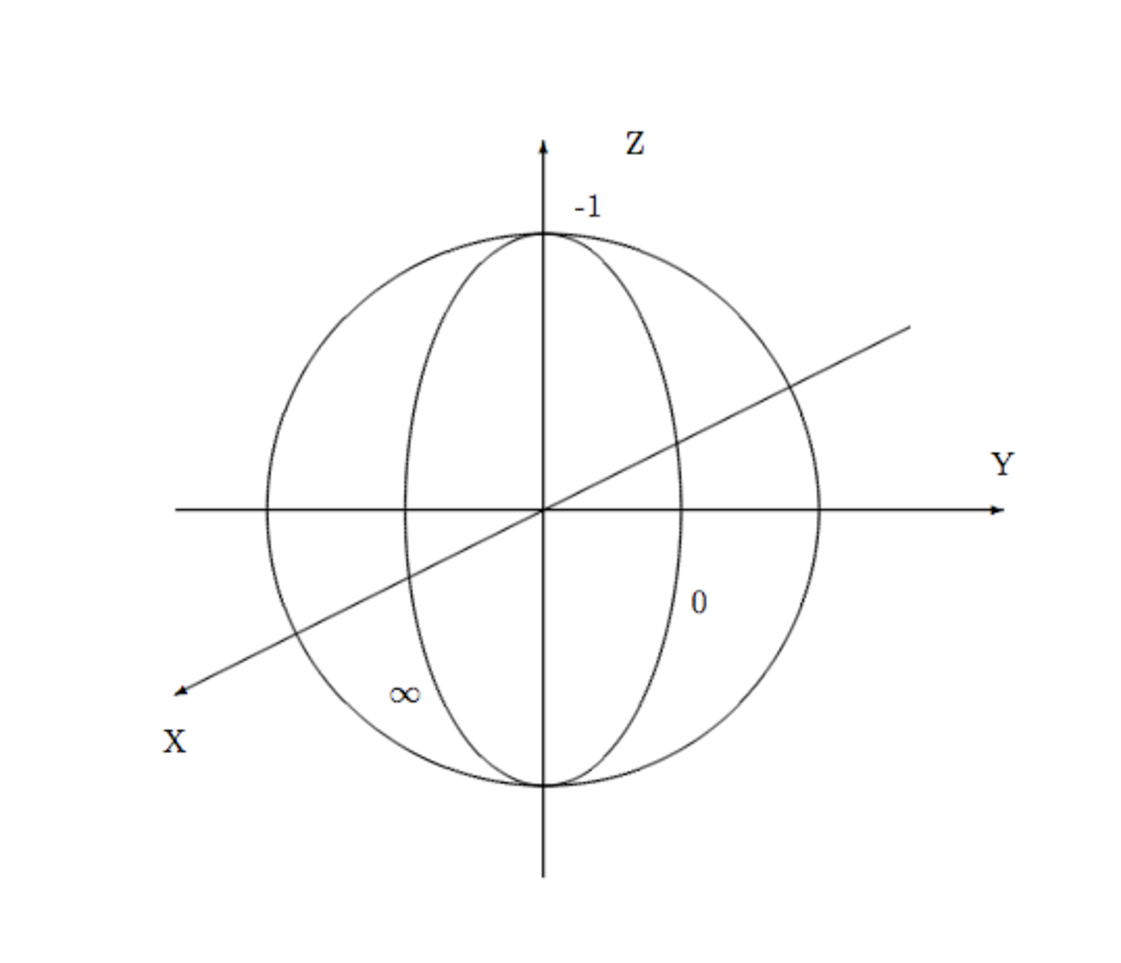
\includegraphics [width=0.6\textwidth]{spherepic.pdf}
\caption{}
\end{center}
\end{figure}

\begin{align*}
&\phi'(\infty) = (\frac{\sqrt{3}}{2}, 0, -\frac{1}{2}), \qquad \phi'(0) = (\frac{-\sqrt{3}}{2}, 0, -\frac{1}{2}), \qquad \phi'(-1) = (0,0,1), \\
&\phi'(\frac{-1}{2} + \frac{\sqrt{3}}{2}i) = (0,1,0), \qquad \phi'(\frac{-1}{2} -\frac{\sqrt{3}}{2}i) = (0,-1,0), \qquad \phi'(1) = (0,0,-1),
\end{align*}
then $\phi' f_4 \phi'^{-1}$ is a counterclockwise rotation about the positive y-axis by angle $\frac{2\pi}{3}$,
and $\phi' f_2 \phi'^{-1}$ is a counterclockwise rotation about the positive z-axis by angle $\pi$.

\begin{lemma}
If $\varphi \in G[\LLL] \setminus \{I \}$ be the automorphism such that $\varphi(Q_{-1}) = Q_{-1}$, then $\varphi = \varphi_2$.
\end{lemma}

\begin{proof}
Let $f \in \MMM$ be the $M\ddot{o}bius$ transform such that $\varphi(Q_z) = Q_{f(z)}$. Then $\phi' f \phi'^{-1}$($\in SO(3)$) will
fix $(0,0,0)$ and $(0,0,1)$, thus $\phi' f \phi'^{-1}$ is a rotation about the z-axis. Let $z_1 = f(\infty)$, $z_2 = f(0)$. Since
$\{Q_{-1}, Q_{z_1}, Q_{z_2} \}$ must be free, we have $z_1$, $z_2$ are in $[0, +\infty)$, then $\phi'(z_1)$ and $\phi'(z_2)$ are
in xz-Plane. and the only non-trivial rotation about the z-axis that map $(\frac{\sqrt{3}}{2}, 0, -\frac{1}{2})$($= \phi'(\infty)$) onto some
point in xz-Plane is $\phi' f_2 \phi'^{-1}$, thus $\varphi = \varphi_2$.
\end{proof}

Let
\begin{align*}
\DDD = \{z | \exists z_1, z_2 \in \C \cup \{\infty \} \mbox{, such that } \{ Q_z, Q_{z_1}, Q_{z_2} \} \mbox{ are 3 free projections} \}.
\end{align*}

\begin{corollary}
For any $z \in \DDD$, there exist one and only one $\varphi \in G[\LLL] \setminus \{I \}$ such that $\varphi(Q_z) = Q_z$.
\end{corollary}

\begin{corollary}
$\phi' \MMM[\LLL] \phi'^{-1} \subsetneq SO(3)$.
\end{corollary}

\begin{proof}
If $\phi' \MMM[\LLL] \phi'^{-1} = SO(3)$, then $\DDD = \C \cup \{\infty \}$, but $\frac{-1}{2} + \frac{\sqrt{3}}{2}i \notin \DDD$ since
$\varphi_4$ and $\varphi_{4}^{2}$ are fix $Q_{\frac{-1}{2} + \frac{\sqrt{3}}{2}i}$.
\end{proof}

\begin{lemma}
$\MMM[\LLL]$ is a closed subgroup of $\G$. Thus $\phi' \MMM[\LLL] \phi'^{-1}$ is a closed subgroup of $SO(3)$.
\end{lemma}

\begin{proof}
The topology on $\G$ is induce by the following metric
\begin{align*}
\sigma(f,g) = sup_{z \in \widehat{\C}}d(f(z), g(z)),
\end{align*}
where $d$ is the chordal metric on $\widehat{\C}$.
Let $g_1$, $g_2 \ldots$ be $M\ddot{o}bius$ transformations in $\MMM[\LLL]$ such that $g_n \rightarrow g$.
Let $z_{1}^{n} = g_n(\infty)$, $z_{2}^{n} = g_n(0)$, $z_{3}^{n} = g_n(-1)$, we know that $\{Q_{z_{1}^{n}}, Q_{z_{2}^{n}},
Q_{z_{3}^{n}} \}$ are free projection for each $n$. Also denote $g(\infty)$, $g(0)$, $g(-1)$ by $z_1$, $z_2$, $z_3$ respectively.
If we can show $\{Q_{z_{1}}, Q_{z_{2}},Q_{z_{3}} \}$ are free projections, then $g \in \MMM[\LLL]$ since there will be an
automorphism $\phi$, such that $\phi(Q_{\infty}) = Q_{z_1}$, $\phi(Q_{0}) = Q_{z_2}$, $\phi(Q_{-1}) = Q_{z_3}$.

Because $\sigma(g_n,g) \rightarrow 0$, we have $d(z_i, z^{n}_{i}) \rightarrow 0$, $i = 1$, $2$, $3$, this implies
\begin{align*}
\|Q_{z_i} - Q_{z^{n}_{i}}\|_2 \rightarrow 0, \qquad i = 1, 2, 3.
\end{align*}
Then by Cauchy-Schwarz inequality (also note that the product of projections has norm less then $1$), it is not hard to see that
each joint moment of $\{Q_{z_{1}^{n}}, Q_{z_{2}^{n}},Q_{z_{3}^{n}} \}$ converges
towards the corresponding joint moment of $\{Q_{z_{1}}, Q_{z_{2}},Q_{z_{3}} \}$
(we only need to consider the joint moment because the random variables here are all
projections). Thus $\{Q_{z_{1}^{n}}, Q_{z_{2}^{n}},Q_{z_{3}^{n}} \}$ converges in
distribution towards $\{Q_{z_{1}}, Q_{z_{2}},Q_{z_{3}} \}$, and $\{Q_{z_{1}}, Q_{z_{2}},Q_{z_{3}} \}$ are free.
\end{proof}

The closed subgroups of $SO(3)$ are cyclic groups $C_n$, dihedral groups $D_n$, tetrahedral group $T$, octahedral group
$O$, the icosahedral group $Y$, and two infinite closed subgroups $C_{\infty} \thickapprox SO(2)$ generated by an arbitrary
rotation around an axis and $D_{\infty}$ which is generated by $C_{\infty}$ and a rotation $\pi$ around an axis orthogonal to
the axis of rotation of $C_{\infty}$.

Since $D_{3} \subset \phi' \MMM[\LLL] \phi'^{-1}$, so $\phi' \MMM[\LLL] \phi'^{-1}$ can not be $C_n$ and $C_{\infty}$, which are both
Abelian.

\begin{lemma}
$\phi' \MMM[\LLL] \phi'^{-1} \neq D_n$, for $n \geq 4$.
\end{lemma}

\begin{proof}
Assume that $\phi' \MMM[\LLL] \phi'^{-1} = D_n$ for $n \geq 4$. Since $D_3 \subset \phi' \MMM[\LLL] \phi'^{-1}$, then $n$ must divide $3$ or $n = \infty$.
For any $\theta \in [0, 2\pi]$, let $T_{\theta} = \phi'^{-1}T_{\theta}' \phi' \in \MMM[\LLL]$, where $T_{\theta}' \in SO(3)$ is the
counterclockwise rotation about the positive y-axis by angle $\theta$:
\begin{align*}
T_{\theta}'((x,y,t)) = \left(
                         \begin{array}{ccc}
                           cos(\theta) & 0 & sin(\theta) \\
                           0 & 1 & 0 \\
                           -sin(\theta) & 0 & cos(\theta) \\
                         \end{array}
                       \right)\left(
                                \begin{array}{c}
                                  x \\
                                  y \\
                                  t \\
                                \end{array}
                              \right).
\end{align*}
Direct computation will give
\begin{align*}
T_{\theta}(\infty) = \frac{sin(\frac{\theta}{2} + \frac{2\pi}{3})}{sin(\frac{\theta}{2})},
T_{\theta}(0) = \frac{sin(\frac{\theta}{2})}{sin(\frac{\theta}{2} - \frac{2\pi}{3})},
T_{\theta}(-1) = \frac{sin(\frac{\theta}{2} + \frac{2\pi}{3})+ sin(\frac{\theta}{2})}{sin(\frac{\theta}{2} - \frac{2\pi}{3}) + sin(\frac{\theta}{2})}.
\end{align*}
Next we will show that for any $\theta \in (\frac{2\pi}{3}, \frac{4\pi}{3})$, $T_{\theta} \notin \MMM[\LLL]$. This will end the proof,
since for any $\theta \notin \{\frac{2\pi}{3}, \frac{4\pi}{3} , 0 \}$, there exist $n \in \N$, such that $n\theta$ $mod$ $2\pi \in
(\frac{2\pi}{3}, \frac{4\pi}{3})$.

Fix any $\theta \in (\frac{2\pi}{3}, \frac{4\pi}{3})$, if $T_{\theta} \in \MMM[\LLL]$, let $T_{\theta}(0) = z_1$,
$T_{\theta}(\infty) = z_2$, $T_{\theta}(-1) = z_3$. By the computation in the proof of Lemma 4.1, we have
\begin{align*}
&(I - Q_{\infty}WQ_{z_1}WQ_{\infty})^{-1}[Q_{\infty}WQ_{z_1}W(I-Q_{\infty})] \\
 & \qquad -(I - Q_{\infty}WQ_{z_3}WQ_{\infty})^{-1}[Q_{\infty}WQ_{z_3}W(I-Q_{\infty})] \\
 & \qquad = (\frac{1}{z_1 - z_2} - \frac{1}{z_3 - z_2})\frac{I}{\sqrt{I - K_{z_2}}}U_{z_2}S^{-1}\frac{I}{\sqrt{I - K_{z_2}}}U_{z_2}\\
 & \qquad = -\frac{4}{3}sin^{2}(\frac{\theta}{2})\frac{I}{\sqrt{I - K_{z_2}}}U_{z_2}S^{-1}\frac{I}{\sqrt{I - K_{z_2}}}U_{z_2},
\end{align*}
where $W$ is defined in the proof of Lemma 4.1.
Since $\{WQ_{z_2}W = Q_{\infty}, WQ_{z_1}W, WQ_{z_3}W \}$ are free, we must have
\begin{align*}
L(-\frac{4}{3}sin^{2}(\frac{\theta}{2})\frac{I}{\sqrt{I - K_{z_2}}}U_{z_2}S^{-1}\frac{I}{\sqrt{I - K_{z_2}}}U_{z_2}) = L(S),
\end{align*}
where
\begin{align*}
L(a) = log\Delta(a) = \int^{\infty}_{0} log t d_{\mu_{|a|}(t)} \in [-\infty, \infty[
\end{align*}
($\Delta$ is the Fuglede-Kadison-determinant on $(\LLL'', \tau)$).
Thus we have
\begin{align*}
L(S) &= L(-\frac{4}{3}sin^{2}(\frac{\theta}{2})) + 2L(\frac{I}{\sqrt{I - K_{z_2}}}U_{z_2}) + L(S^{-1})\\
     &= log(\frac{4}{3}sin^{2}(\frac{\theta}{2})) + 2L(\frac{I}{\sqrt{I - K_{z_2}}}) - L(S),
\end{align*}
which implies that
\begin{align*}
2L(S) = log(\frac{4}{3}sin^{2}(\frac{\theta}{2})) + 2L(\frac{I}{\sqrt{I - K_{z_2}}}).
\end{align*}
We already know for all $\theta \in [\frac{2\pi}{3}, \frac{4\pi}{3}]$,
\begin{align*}
L(\frac{I}{\sqrt{I - K_{z_2}}}) = L(\frac{I}{\sqrt{I - K_{0}}}),
\end{align*}
and if $\theta = \frac{2\pi}{3}$, $\frac{4}{3}sin^{2}(\frac{\theta}{2}) = 1$,
\begin{align*}
L(S) = L(\frac{I}{\sqrt{I - K_{0}}}),
\end{align*}
thus we have $log(\frac{4}{3}sin^{2}(\frac{\theta}{2})) = 0$, and this is impossible for $\theta \in (\frac{2\pi}{3}, \frac{4\pi}{3})$.
\end{proof}

\begin{remark}
Actually, we can check $L(S) = L(\frac{I}{\sqrt{I - K_{-1}}})$ explicitly. By the same method in the proof of lemma 2.1,
we have
\begin{align*}
d_{\mu_{|S|}}(t) = \frac{4}{\pi} \frac{1}{t^2 + 4} 1_{(0, +\infty)}(t)dt.
\end{align*}
So a application of residue formula(\cite{SS} Chapter3 Exercises 10) will give
\begin{align*}
L(S) = \frac{4}{\pi}\int_{0}^{\infty} \frac{log t}{t^2 + 4} dt = log2.
\end{align*}
Now we need to show $L(\frac{I}{\sqrt{I - K_{0}}}) = log2$. Because
$d_{\mu_{\sqrt{\frac{K_{-1}}{I - K_{0}}}}}(t) = \frac{2}{\pi} \frac{1}{t^2 + 1} 1_{(0, +\infty)}(t)dt$,
we have
\begin{align*}
d_{\mu_{\sqrt{\frac{I}{I - K_{0}}}}}(t) = \frac{2}{\pi} \frac{1}{t\sqrt{t^2 - 1}} 1_{(1, +\infty)}(t)dt.
\end{align*}
Then we know
\begin{align*}
L(\frac{I}{\sqrt{I - K_{0}}}) &= \frac{2}{\pi} \int_{1}^{+\infty} \frac{log t}{t\sqrt{t^2 - 1}} 1_{(1, +\infty)}(t)dt \\
                               &= \frac{1}{\pi} \int_{0}^{+\infty} \frac{log(x^2+1)}{x^2 + 1} dx, \qquad (t = \sqrt{x^2 + 1}),\\
                               &= -\frac{2}{\pi} \int_{0}^{\frac{\pi}{2}} log(cos \theta) d\theta. \qquad (x = tg \theta).
\end{align*}
The last integral is computed in \cite{MR} by rewriting it as
\begin{align*}
\int_{0}^{\frac{\pi}{2}} log(cos \theta) d\theta &= -\frac{1}{4} \int_{0}^{1} log t \frac{1}{\sqrt{t}\sqrt{1-t}}\\
                                                 &= \frac{1}{4} \frac{\partial}{\partial \beta} \int_{0}^{1} t^{\beta - \frac{1}{2}}(1-t)^{\alpha - \frac{1}{2}} |_{\alpha = \beta = 0} \\
                                                 & = \frac{\pi}{4} \frac{\partial}{\partial \beta} [\frac{\Gamma(\frac{1}{2} + \alpha)\Gamma(\frac{1}{2} + \beta)}{\Gamma(1 + \alpha + \beta)\Gamma^{2}(\frac{1}{2})}]|_{\alpha = \beta = 0} = -\frac{\pi}{2}log2.
\end{align*}
\end{remark}

\begin{remark}[Shortcut]
Since
\begin{align*}
L(I - K_z) &= \frac{1}{\pi}\int^{1}_{0} log(t)\frac{\Delta}{\sqrt{t(1-t)}(1 + (\Delta^2 -1)t)}dt\\
           &= -\frac{2}{\pi}\int^{+\infty}_{0}log(t^{2} + 1)\frac{\Delta}{t^{2} + \Delta^{2}}dt  = -2log(\Delta + 1),
\end{align*}
where $\Delta = |z| + |z + 1|$. Then
\begin{align*}
L(I - (WQ_zW)_{1,1}) &= 2log(|z_2 - z|) + L(I - K_{z}) + L(I - K_{z_2}) + 2L(S)\\
                     &= 2log(|z_2 - z|) + 2log(2) - 2log(1 + |z| + |z+1|) - 2log(1 + |z_2| + |z_2 +1|) \\
                     &= 2log(\frac{2|z_2 - z|}{(1 + |z| + |z+1|)(1 + |z_2| + |z_2 + 1|)}).
\end{align*}
Note by the facts in section 3, we will know the fact we want immediately.
\end{remark}

\begin{lemma}
$\phi' \MMM[\LLL] \phi'^{-1} \neq T$.
\end{lemma}

\begin{proof}
Since $T \approx A_4$, the alternating subgroup of $S_4$, and $A_4$ has no subgroup of order 6. This contradict with the
fact that $S_3 \subset \phi' \MMM[\LLL] \phi'^{-1}$.
\end{proof}

Because both $O$ and $Y$ contains $S_3$ as subgroup, we need to find out if $\phi' \MMM[\LLL] \phi'^{-1}$ could
be one of them.

First consider $O$. $O$ is the symmetry group of the cube. We can write down a permutation representation of
the symmetric group on four letters that indicates the group action on the vertices of the cube. If we label
the vertices of the cube as in the picture below, we have

\begin{figure}[H]
\begin{center}
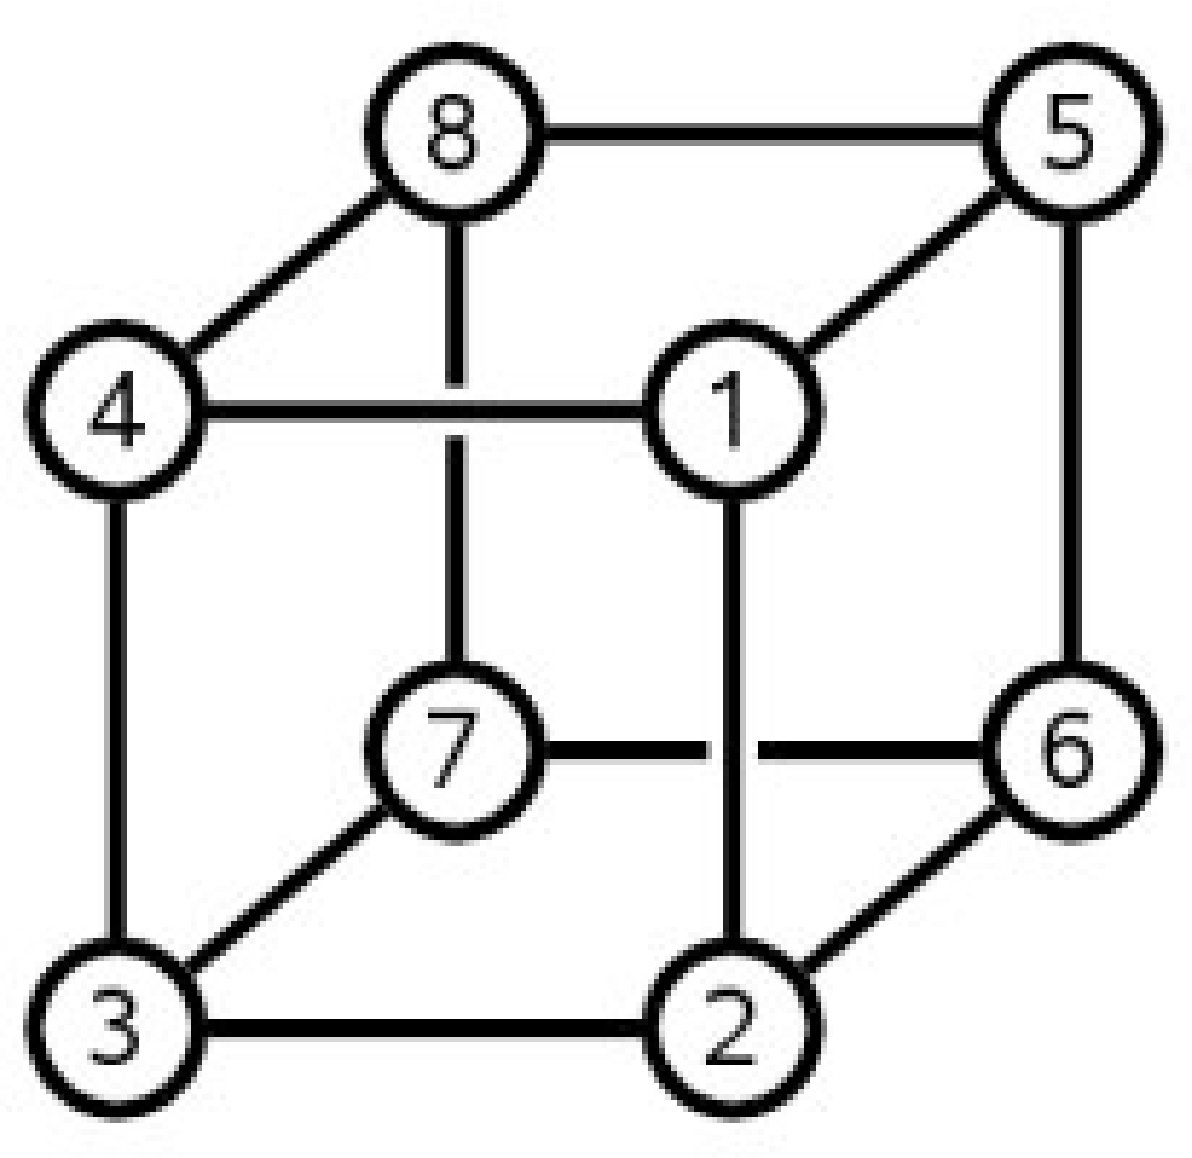
\includegraphics [width=0.4\textwidth]{cube.pdf}
\caption{}
\end{center}
\end{figure}

\begin{align*}
r = (1,2)(3,5)(4,6)(7,8), \qquad s = (1,2,3,4)(5,6,7,8),
\end{align*}
and $r^2 = id$, $s^4 = id$, $(rs)^3 = (2,5,4)(3,6,8) = id$. By the symmetry, we know that
a group element of $O$ is a rotation by $120^\circ$, if and only if it is a rotation about
the line passing through two opposite vertices, for instance vertices 1 and 7 (and there are
8 rotations by $120^\circ$). Also there are six rotation by $180^\circ$ about a 2-fold axis,
i.e. the rotation by $180^\circ$ about the line passing through the midpoint of opposite edges
(for example edge (1,2) and edge (8,7)).

Next we assume the coordinate of the vertices of the cube in Figure 1 is
\begin{align*}
&(1) = (\frac{\sqrt{3}}{3},\frac{\sqrt{3}}{3}, \frac{\sqrt{3}}{3}); \qquad (4) = (\frac{\sqrt{3}}{3},-\frac{\sqrt{3}}{3}, \frac{\sqrt{3}}{3});\\
&(5) = (-\frac{\sqrt{3}}{3},\frac{\sqrt{3}}{3}, \frac{\sqrt{3}}{3}); \qquad (8) = (-\frac{\sqrt{3}}{3},-\frac{\sqrt{3}}{3}, \frac{\sqrt{3}}{3});\\
&(2) = (\frac{\sqrt{3}}{3},\frac{\sqrt{3}}{3}, -\frac{\sqrt{3}}{3}); \qquad (3) = (\frac{\sqrt{3}}{3},-\frac{\sqrt{3}}{3}, -\frac{\sqrt{3}}{3});\\
&(6) = (-\frac{\sqrt{3}}{3},\frac{\sqrt{3}}{3}, -\frac{\sqrt{3}}{3}); \qquad (7) = (-\frac{\sqrt{3}}{3},-\frac{\sqrt{3}}{3}, -\frac{\sqrt{3}}{3}).\\
\end{align*}

We will map $(0,1,0)$ to $(\frac{\sqrt{3}}{3},\frac{\sqrt{3}}{3}, \frac{\sqrt{3}}{3})$.

Let
\begin{align*}
T = \left(
      \begin{array}{ccc}
        -\frac{1}{\sqrt{6}} & \frac{1}{\sqrt{3}} & -\frac{1}{\sqrt{2}} \\
        -\frac{1}{\sqrt{6}} & \frac{1}{\sqrt{3}} & \frac{1}{\sqrt{2}} \\
        \frac{2}{\sqrt{6}} & \frac{1}{\sqrt{3}} & 0 \\
      \end{array}
    \right), \qquad
A_{x} = \left(
          \begin{array}{ccc}
            1 & 0 & 0 \\
            0 & -1 & 0 \\
            0 & 0 & -1 \\
          \end{array}
        \right),
\end{align*}
then
\begin{align*}
T^{-1}A_{x}T\left(
              \begin{array}{c}
                0 \\
                0 \\
                1 \\
              \end{array}
            \right)
= \left(
    \begin{array}{c}
      \frac{\sqrt{3}}{3} \\
      -\frac{\sqrt{6}}{3} \\
      0 \\
    \end{array}
  \right),
T^{-1}A_{x}T\left(
              \begin{array}{c}
                \frac{\sqrt{3}}{2} \\
                0 \\
                -\frac{1}{2} \\
              \end{array}
            \right)
= \left(
    \begin{array}{c}
      -\frac{\sqrt{3}}{2} \\
      0 \\
      \frac{1}{2} \\
    \end{array}
  \right),
T^{-1}A_{x}T\left(
              \begin{array}{c}
                -\frac{\sqrt{3}}{2} \\
                0 \\
                -\frac{1}{2} \\
              \end{array}
            \right)
= \left(
    \begin{array}{c}
      \frac{\sqrt{3}}{6} \\
      \frac{\sqrt{6}}{3}  \\
      -\frac{1}{2} \\
    \end{array}
  \right).
\end{align*}
Let
\begin{align*}
z_1 &= \phi'^{-1}( \frac{\sqrt{3}}{3}, -\frac{\sqrt{6}}{3}, 0 ) = -1 - \sqrt{2}i; \\
z_2 &= \phi'^{-1}((\frac{-\sqrt{3}}{2},0,\frac{1}{2})) = -\frac{1}{2};\\
z_3 &= \phi'^{-1}((\frac{\sqrt{3}}{6}, \frac{\sqrt{6}}{3}, -\frac{1}{2})) = \sqrt{2}i.
\end{align*}
By the same method we used in the proof of Lemma 4.5, the following fact tells us that $\phi' \MMM[\LLL] \phi'^{-1} \neq O$.
\begin{align*}
|\frac{1}{z_1 - z_2} - \frac{1}{z_3 - z_2}| = |\frac{1}{-\frac{1}{2} - \sqrt{2}i} - \frac{1}{\frac{1}{2}+ \sqrt{2}i}| = |\frac{2}{\frac{1}{2}+ \sqrt{2}i}| = \frac{4}{3} \neq 1.
\end{align*}

Next we will consider $Y$. $Y$ is the symmetry group of the regular icosahedron.

\begin{figure}[H]
\begin{center}
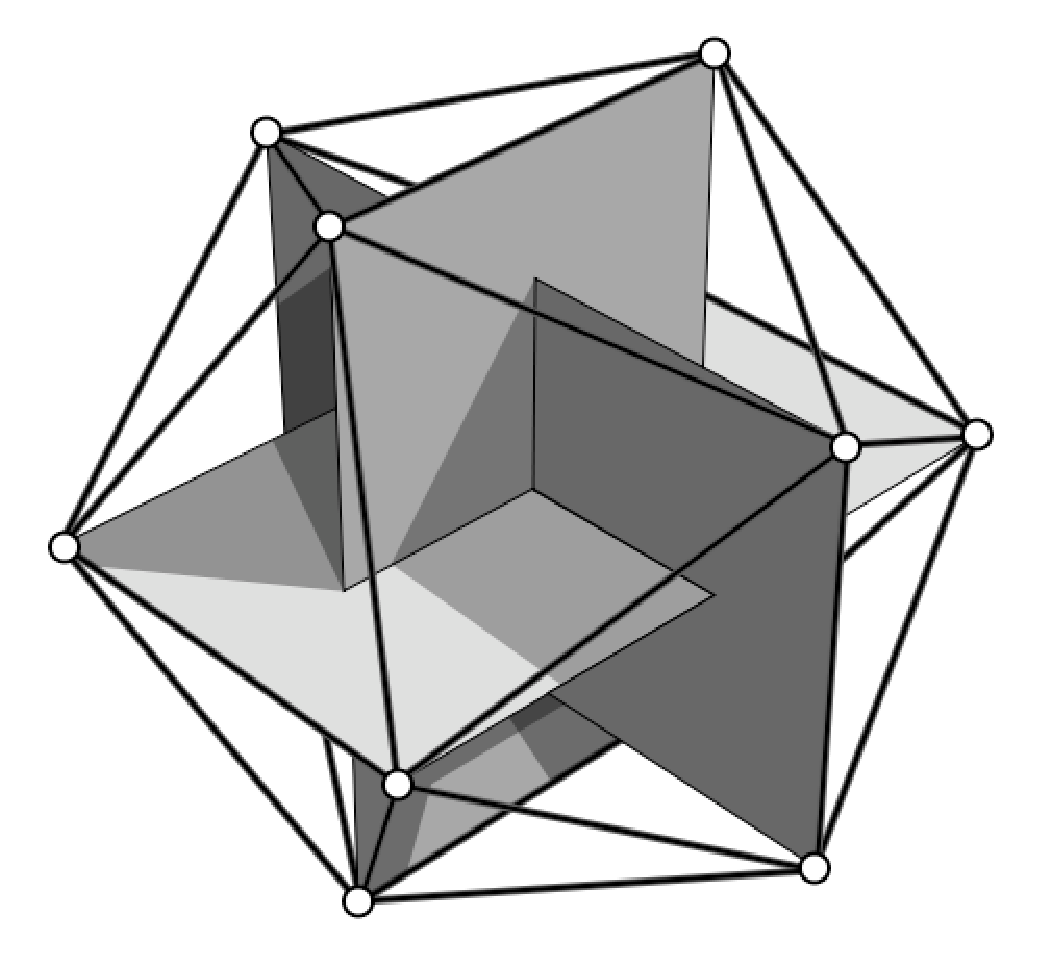
\includegraphics [width=0.5\textwidth]{Icosahedron.pdf}
\caption{}
\end{center}
\end{figure}

In the group above, we use Cartesian coordinates define the vertices of an icosahedron:
\begin{align*}
(\pm 1, 0 , \pm \frac{1 + \sqrt{5}}{2}); \qquad (0, \pm \frac{1 + \sqrt{5}}{2}, \pm 1); \qquad (\pm \frac{1 + \sqrt{5}}{2},\pm 1, 0).
\end{align*}

Let
\begin{align*}
T = \left(
      \begin{array}{ccc}
        \frac{-2 - \sqrt{5}}{\sqrt{42 + 18\sqrt{5}}} & \frac{1 + \sqrt{5}}{\sqrt{42 + 18\sqrt{5}}} & \frac{-2 - \sqrt{5}}{\sqrt{14 + 6\sqrt{5}}} \\
        \frac{1 + \sqrt{5}}{2\sqrt{42 + 18\sqrt{5}}} & \frac{4 + 2\sqrt{5}}{\sqrt{42 + 18\sqrt{5}}} & \frac{1 + \sqrt{5}}{2\sqrt{14 + 6\sqrt{5}}} \\
        \frac{\sqrt{3}}{2} & 0 & -\frac{1}{2} \\
      \end{array}
    \right),
\end{align*}
we have
\begin{align*}
T\left(
   \begin{array}{c}
     0 \\
     1 \\
     0 \\
   \end{array}
 \right)=
 \left(
   \begin{array}{c}
     \sqrt{\frac{1}{6}(3 - \sqrt{5})} \\
     \sqrt{\frac{1}{6}(3 + \sqrt{5})}\\
     0 \\
   \end{array}
 \right), \qquad
 T\left(
   \begin{array}{c}
     \frac{\sqrt{3}}{2} \\
     0 \\
     -\frac{1}{2} \\
   \end{array}
 \right)=
 \left(
   \begin{array}{c}
     0\\
     0\\
     1 \\
   \end{array}
 \right).
\end{align*}
If we assume that $\phi' \MMM[\LLL] \phi'^{-1} \thickapprox Y$, we know the rotation by $180^{\circ}$ about $ \left(
   \begin{array}{c}
     0\\
     0\\
     1 \\
   \end{array}
 \right)$ and the rotation by $120^{\circ}$ about $ \left(
   \begin{array}{c}
     \sqrt{\frac{1}{6}(3 - \sqrt{5})} \\
     \sqrt{\frac{1}{6}(3 + \sqrt{5})}\\
     0 \\
   \end{array}
 \right)$ are in $T\phi' \MMM[\LLL] \phi'^{-1}T^{-1}$, thus
\begin{align*}
A_x = T^{-1}\left(
   \begin{array}{ccc}
     1 & 0 & 0 \\
     0 & -1 & 0 \\
     0 & 0 & -1 \\
   \end{array}
 \right)T =
 \left(
   \begin{array}{ccc}
     \frac{-9 + \sqrt{5}}{12} & -\frac{1}{3} & \sqrt{\frac{7}{24} + \frac{\sqrt{5}}{8}} \\
     -\frac{1}{3} & -\frac{\sqrt{5}}{3} & -\frac{1}{\sqrt{3}} \\
      \sqrt{\frac{7}{24} + \frac{\sqrt{5}}{8}}& -\frac{1}{\sqrt{3}} & \frac{-1 + \sqrt{5}}{4} \\
   \end{array}
 \right) \in \phi' \MMM[\LLL] \phi'^{-1}.
\end{align*}

Thus
\begin{align*}
A_x \left(
      \begin{array}{c}
        \frac{\sqrt{3}}{2} \\
        0 \\
        -\frac{1}{2} \\
      \end{array}
    \right)
    =\left(
      \begin{array}{c}
        -\frac{\sqrt{3}}{2} \\
        0 \\
        \frac{1}{2} \\
      \end{array}
    \right),
A_x \left(
      \begin{array}{c}
        0 \\
        0 \\
        1 \\
      \end{array}
    \right)
    =\left(
      \begin{array}{c}
       \sqrt{\frac{7}{24} + \frac{\sqrt{5}}{8}} \\
        -\frac{1}{\sqrt{3}} \\
       \frac{-1 + \sqrt{5}}{4} \\
      \end{array}
    \right),
A_x \left(
      \begin{array}{c}
        -\frac{\sqrt{3}}{2} \\
        0 \\
        -\frac{1}{2} \\
      \end{array}
    \right)
    =\left(
      \begin{array}{c}
        \frac{3-\sqrt{5}}{4\sqrt{3}} \\
        \frac{1}{\sqrt{3}} \\
        \frac{-1-\sqrt{5}}{4} \\
      \end{array}
    \right).
\end{align*}
Then
\begin{align*}
z_1 &= \phi'^{-1}( \left(
      \begin{array}{c}
       \sqrt{\frac{7}{24} + \frac{\sqrt{5}}{8}} \\
        -\frac{1}{\sqrt{3}} \\
       \frac{-1 + \sqrt{5}}{4} \\
      \end{array}
    \right) ) = -\frac{1}{2} - \frac{1}{2}(\sqrt{5} + 2i); \\
z_2 &= \phi'^{-1}(\left(
      \begin{array}{c}
        -\frac{\sqrt{3}}{2} \\
        0 \\
        \frac{1}{2} \\
      \end{array}
    \right)) = -\frac{1}{2};\\
z_3 &= \phi'^{-1}(\left(
      \begin{array}{c}
        \frac{3-\sqrt{5}}{4\sqrt{3}} \\
        \frac{1}{\sqrt{3}} \\
        \frac{-1-\sqrt{5}}{4} \\
      \end{array}
    \right)) = -\frac{1}{2} + \frac{1}{2}(\sqrt{5} + 2i),
\end{align*}
and we also have
\begin{align*}
|\frac{1}{z_1 - z_2} - \frac{1}{z_3 - z_2}| = |\frac{1}{- \frac{1}{2}(\sqrt{5} + 2i)} - \frac{1}{\frac{1}{2}(\sqrt{5} + 2i)}|
= |\frac{4}{\sqrt{5} + 2i}| = \frac{4}{3} \neq 1.
\end{align*}

The conclusions of the above argument are summarized in the following result.

\begin{theorem}
 $\phi' \MMM[\LLL] \phi'^{-1} \thickapprox S_3 $
\end{theorem}

\section{derivative}
Remember that
\begin{align*}
\sqrt{K_{z}(I-K_{z})^{-1}}U_{z} = &(1+z)\sqrt{H_{1}(I-H_{1})^{-1}}-
                                   z\sqrt{H_{2}(I-H_{2})^{-1}}V \\
                                 &=zS + \sqrt{H_{1}(I-H_{1})^{-1}},
\end{align*}
where $S = \sqrt{\frac{H_1}{I - H_1}} - \sqrt{\frac{H_2}{I - H_2}}V$.
Let
\begin{align*}
F(z) = |z|^{2}SS^{*} + zS\sqrt{\frac{H_1}{I - H_1}} + \overline{z}\sqrt{\frac{H_1}{I - H_1}}S^{*} + \frac{H_1}{I - H_1};\\
G(z) = |z|^{2}S^{*}S + z\sqrt{\frac{H_1}{I - H_1}}S + \overline{z}S^{*}\sqrt{\frac{H_1}{I - H_1}} + \frac{H_1}{I - H_1},
\end{align*}
then we have
\begin{align*}
K_{z} = I - (I + F(z))^{-1}; \qquad
U_{z}^{*}(I - K_z)U_{z} = (I + G(z))^{-1}.
\end{align*}
And simple calculation will give (below we treat $K_{z}$ as operator valued function and $z = x + iy$):
\begin{align*}
&\frac{\partial K_{z}}{\partial x} = (I + F(z))^{-1}(2xSS^{*} + S\sqrt{\frac{H_1}{I - H_1}} + \sqrt{\frac{H_1}{I - H_1}}S^{*})(I + F(z))^{-1};\\
&\frac{\partial K_{z}}{\partial y} = (I + F(z))^{-1}[2ySS^{*} + i(S\sqrt{\frac{H_1}{I - H_1}} - \sqrt{\frac{H_1}{I - H_1}}S^{*})](I + F(z))^{-1};\\
&\frac{\partial \sqrt{K_{z}(I-K_z)}U_z}{\partial x} = - \frac{\partial K_{z}}{\partial x}\sqrt{\frac{K_{z}}{(I-K_{z})}}U_{z} + (I - K_z)S;\\
&\frac{\partial \sqrt{K_{z}(I-K_z)}U_z}{\partial y} = - \frac{\partial K_{z}}{\partial y}\sqrt{\frac{K_{z}}{(I-K_{z})}}U_{z} + i(I - K_z)S;\\
&\frac{\partial U_{z}^{*}\sqrt{K_{z}(I-K_z)}}{\partial x} = - U_{z}^{*}\sqrt{\frac{K_{z}}{(I-K_{z})}}\frac{\partial K_{z}}{\partial x} + S^{*}(I - K_z) = (\frac{\partial \sqrt{K_{z}(I-K_z)}U_z}{\partial x})^{*};\\
&\frac{\partial U_{z}^{*}\sqrt{K_{z}(I-K_z)}}{\partial y} = - U_{z}^{*}\sqrt{\frac{K_{z}}{(I-K_{z})}}\frac{\partial K_{z}}{\partial y} - iS^{*}(I - K_z) = (\frac{\partial \sqrt{K_{z}(I-K_z)}U_z}{\partial y})^{*};\\
&\frac{\partial U_{z}^{*}(I - K_{z})U_{z}}{\partial x} = -(I + G(z))^{-1}(2xS^{*}S + \sqrt{\frac{H_1}{I - H_1}}S + S^{*}\sqrt{\frac{H_1}{I - H_1}})(I + G(z))^{-1};\\
&\frac{\partial U_{z}^{*}(I - K_{z})U_{z}}{\partial y} = -(I + G(z))^{-1}[2yS^{*}S + i(\sqrt{\frac{H_1}{I - H_1}}S - S^{*}\sqrt{\frac{H_1}{I - H_1}})](I + G(z))^{-1}.\\
\end{align*}
Since
\begin{align*}
\frac{\partial}{\partial z} = \frac{1}{2}[\frac{\partial}{\partial x} -i\frac{\partial}{\partial y}]; \qquad
\frac{\partial}{\partial \overline{z}} = \frac{1}{2}[\frac{\partial}{\partial x} + i\frac{\partial}{\partial y}],
\end{align*}
we have
\begin{align*}
\frac{\partial Q_{z}}{\partial z} &=
\left(
                                      \begin{array}{cc}
                                         \begin{array}{c}
                                           (I + F(z))^{-1}(\overline{z}SS^{*}  \\
                                           \qquad \qquad + S\sqrt{\frac{H_1}{I - H_1}})(I + F(z))^{-1}
                                         \end{array}
                                         & \begin{array}{c}
                                             (I - K_z)S-(I + F(z))^{-1}(\overline{z}SS^{*}   \\
                                             \qquad \qquad + S\sqrt{\frac{H_1}{I - H_1}})(I + F(z))^{-1}\sqrt{\frac{K_{z}}{(I-K_{z})}}U_{z}
                                           \end{array}
                                          \\
                                        \begin{array}{c}
                                        -U_{z}^{*}\sqrt{\frac{K_{z}}{(I-K_{z})}}(I + F(z))^{-1}(\overline{z}SS^{*}  \\
                                         \qquad \qquad  + S\sqrt{\frac{H_1}{I - H_1}})(I + F(z))^{-1}
                                        \end{array}
                                        & \begin{array}{c}
                                          - (I + G(z))^{-1}(\overline{z}S^{*}S  \\
                                             \qquad \qquad + \sqrt{\frac{H_1}{I - H_1}}S )(I + G(z))^{-1}
                                          \end{array}
                                         \\
                                      \end{array}
                                    \right)\\
                                    &=\left(
                                      \begin{array}{cc}
                                         \begin{array}{c}
                                           (I - K_z)(\overline{z}SS^{*}  \\
                                           \qquad \qquad + S\sqrt{\frac{H_1}{I - H_1}})(I - K_z)
                                         \end{array}
                                         & \begin{array}{c}
                                             (I - K_z)S-(I - K_z)(\overline{z}SS^{*}   \\
                                             \qquad \qquad + S\sqrt{\frac{H_1}{I - H_1}})\sqrt{K_{z}(I-K_{z})}U_{z}
                                           \end{array}
                                          \\
                                        \begin{array}{c}
                                        -U_{z}^{*}\sqrt{K_{z}(I-K_{z})}(\overline{z}SS^{*}  \\
                                         \qquad \qquad  + S\sqrt{\frac{H_1}{I - H_1}})(I - K_z)
                                        \end{array}
                                        & \begin{array}{c}
                                            -U^{*}_{z}(I - K_z)U_{z}(\overline{z}S^{*}S  \\
                                             \qquad \qquad + \sqrt{\frac{H_1}{I - H_1}}S )U^{*}_{z}(I - K_z)U_{z}
                                          \end{array}
                                         \\
                                      \end{array}
                                    \right)\\
                                    &=\left(
                                       \begin{array}{cc}
                                         (I-K_z) & 0 \\
                                         0 & U^{*}_{z}\sqrt{K_{z}(I-K_{z})} \\
                                       \end{array}
                                     \right) \times
                                     \left(
                                       \begin{array}{cc}
                                         S & S \\
                                         -S & -S \\
                                       \end{array}
                                     \right)\times
                                     \left(
                                       \begin{array}{cc}
                                         U^{*}_{z}\sqrt{K_{z}(I-K_{z})} & 0 \\
                                         0 & U^{*}_{z}(I- K_{z})U_z \\
                                       \end{array}
                                     \right)
\end{align*}
\begin{align*}
\frac{\partial Q_{z}}{\partial \overline{z}} &=
\left(
                                      \begin{array}{cc}
                                         \begin{array}{c}
                                           (I + F(z))^{-1}(zSS^{*}  \\
                                           \qquad \qquad + \sqrt{\frac{H_1}{I - H_1}}S^{*})(I + F(z))^{-1}
                                         \end{array}
                                         & \begin{array}{c}
                                             -(I + F(z))^{-1}(zSS^{*}+ \sqrt{\frac{H_1}{I - H_1}}S^{*})   \\
                                             \qquad \qquad \times(I + F(z))^{-1}\sqrt{\frac{K_{z}}{(I-K_{z})}}U_{z}
                                           \end{array}
                                          \\
                                        \begin{array}{c}
                                         -U_{z}^{*}\sqrt{\frac{K_{z}}{(I-K_{z})}}(I + F(z))^{-1}(zSS^{*}  \\
                                         \qquad \qquad  + \sqrt{\frac{H_1}{I - H_1}}S^{*})(I + F(z))^{-1} + S^{*}(I - K_z)
                                        \end{array}
                                        & \begin{array}{c}
                                           - (I + G(z))^{-1}(zS^{*}S  \\
                                             \qquad \qquad + S^{*}\sqrt{\frac{H_1}{I - H_1}} )(I + G(z))^{-1}
                                          \end{array}
                                         \\
                                      \end{array}
                                    \right)\\
                                    &=\left(
                                      \begin{array}{cc}
                                         \begin{array}{c}
                                           (I + K_z)(zSS^{*}  \\
                                           \qquad \qquad + \sqrt{\frac{H_1}{I - H_1}}S^{*})(I + K_z)
                                         \end{array}
                                         & \begin{array}{c}
                                             -(I + K_z)(zSS^{*}+ \sqrt{\frac{H_1}{I - H_1}}S^{*})   \\
                                             \qquad \qquad \times\sqrt{K_{z}(I-K_{z})}U_{z}
                                           \end{array}
                                          \\
                                        \begin{array}{c}
                                         -U_{z}^{*}\sqrt{K_{z}(I-K_{z})}(zSS^{*}  \\
                                         \qquad \qquad  + \sqrt{\frac{H_1}{I - H_1}}S^{*})(I + K_z) + S^{*}(I - K_z)
                                        \end{array}
                                        & \begin{array}{c}
                                           - U^{*}_{z}(I - K_z)U_{z}(zS^{*}S  \\
                                             \qquad \qquad + S^{*}\sqrt{\frac{H_1}{I - H_1}} )U^{*}_{z}(I - K_z)U_{z}
                                          \end{array}
                                         \\
                                      \end{array}
                                    \right)\\
                                    &=\left(
                                        \begin{array}{cc}
                                          \sqrt{K_{z}(I - K_z)}U_z & 0 \\
                                          0 & U^{*}_{z}(I - K_z)U_z \\
                                        \end{array}
                                      \right)\times
                                      \left(
                                        \begin{array}{cc}
                                          S^{*} & -S^{*} \\
                                          S^{*} & -S^{*} \\
                                        \end{array}
                                      \right) \times
                                      \left(
                                        \begin{array}{cc}
                                          I- K_z & 0 \\
                                          0 & \sqrt{K_{z}(I - K_z)}U_z \\
                                        \end{array}
                                      \right)
\end{align*}
Note $F(z)$ and $G(z)$ are self joint, we have the following lemma,

\begin{lemma}
$(\frac{\partial Q_{z}}{\partial z})^{*} = \frac{\partial Q_{z}}{\partial \overline{z}}$.
\end{lemma}

\begin{example}
\begin{align*}
&\frac{\partial Q_{z}}{\partial z}|_{z = 0} =
\left(
                                      \begin{array}{cc}
                                         (I-H_1)S\sqrt{H_{1}(I-H_1)}
                                         & (I-H_1)S(I - H_1)
                                          \\
                                        -\sqrt{H_{1}(I-H_1)}S\sqrt{H_{1}(I-H_1)}
                                        & \sqrt{H_{1}(I-H_1)}S(I-H_1)\\
                                      \end{array}
                                    \right)\\
&\frac{\partial Q_{z}}{\partial \overline{z}}|_{z = 0} =
\left(
                                      \begin{array}{cc}
                                         \sqrt{H_{1}(I-H_1)}S^{*}(I - H_1)
                                         & -\sqrt{H_{1}(I-H_1)}S^{*}\sqrt{H_{1}(I-H_1)}
                                          \\
                                       (I-H_1)S^{*}(I-H_1)
                                        & (I-H_1)S^{*}\sqrt{H_{1}(I-H_1)}
                                         \\
                                      \end{array}
                                    \right)
\end{align*}
\end{example}

If the projections $Q_{\infty}$, $Q_{0}$, $Q_{-1}$ in $M_{2n}(\C)$ are in general position, then the map $\varphi(z) = Q_{z}$ gives a 
holomorphic curve in complex Grassmann manifolds $\mathrm{G}_{n, 2n}$. 

Let $U(2n)$ be the unitary group. A smooth map $g : S^{2} \rightarrow U(2n)$ is a harmonic map if and only if it satisfies the following 
equation $($\cite{KU}$)$: 
\begin{align*}
\frac{\partial A_{z} }{\partial \overline{z}}= [A_{z}, A_{\overline{z}}],
\end{align*}
where $A_{z} = \frac{1}{2} g(z)^{-1} \frac{\partial g(z)}{\partial z}$ and $A_{\overline{z}} = \frac{1}{2} g(z)^{-1} \frac{\partial g(z)}{\partial \overline{z}}$.

Let $g(z) = 2Q_{z} - I$. Then we have 
\begin{align*}
A_{z} &= (2Q_{z} - I)\frac{\partial Q_{z}}{\partial z} \\
&= \left(
                                       \begin{array}{cc}
                                         \sqrt{K_z} & \sqrt{I- K_z}U_z \\
                                         U^{*}_z \sqrt{I- K_z} & -U^{*}_{z}\sqrt{K_{z}}U_{z} \\
                                       \end{array}
                                     \right) \times
\left(
                                       \begin{array}{cc}
                                        I & 0 \\
                                        0&-I\\
                                       \end{array}
                                     \right) \times
\left(
                                       \begin{array}{cc}
                                         \sqrt{K_z} & \sqrt{I- K_z}U_z \\
                                         U^{*}_z \sqrt{I- K_z} & -U^{*}_{z}\sqrt{K_{z}}U_{z} \\
                                       \end{array}
                                     \right) \\
&\times \left(
                                       \begin{array}{cc}
                                         (I-K_z) & 0 \\
                                         0 & U^{*}_{z}\sqrt{K_{z}(I-K_{z})} \\
                                       \end{array}
                                     \right) \times
                                     \left(
                                       \begin{array}{cc}
                                         S & S \\
                                         -S & -S \\
                                       \end{array}
                                     \right)\times
                                     \left(
                                       \begin{array}{cc}
                                         U^{*}_{z}\sqrt{K_{z}(I-K_{z})} & 0 \\
                                         0 & U^{*}_{z}(I- K_{z})U_z \\
                                       \end{array}
                                     \right)\\
&=  \left(
                                       \begin{array}{cc}
                                        - (I-K_z) & 0 \\
                                         U^{*}_{z}\sqrt{K_{z}(I-K_{z})} & 0 \\
                                       \end{array}
                                     \right) \times
                                     \left(
                                       \begin{array}{cc}
                                         S & S \\
                                         -S & -S \\
                                       \end{array}
                                     \right)\times
                                     \left(
                                       \begin{array}{cc}
                                         U^{*}_{z}\sqrt{K_{z}(I-K_{z})} & 0 \\
                                         0 & U^{*}_{z}(I- K_{z})U_z \\
                                       \end{array}
                                     \right),
\end{align*}

\begin{align*}
A_{\overline{z}} &= (2Q_{z} - I)\frac{\partial Q_{z}}{\partial \overline{z}} \\
&= \left(
                                       \begin{array}{cc}
                                         \sqrt{K_z} & \sqrt{I- K_z}U_z \\
                                         U^{*}_z \sqrt{I- K_z} & -U^{*}_{z}\sqrt{K_{z}}U_{z} \\
                                       \end{array}
                                     \right) \times
\left(
                                       \begin{array}{cc}
                                        I & 0 \\
                                        0&-I\\
                                       \end{array}
                                     \right) \times
\left(
                                       \begin{array}{cc}
                                         \sqrt{K_z} & \sqrt{I- K_z}U_z \\
                                         U^{*}_z \sqrt{I- K_z} & -U^{*}_{z}\sqrt{K_{z}}U_{z} \\
                                       \end{array}
                                     \right) \\
&\times\left(
                                        \begin{array}{cc}
                                          \sqrt{K_{z}(I - K_z)}U_z & 0 \\
                                          0 & U^{*}_{z}(I - K_z)U_z \\
                                        \end{array}
                                      \right)\times
                                      \left(
                                        \begin{array}{cc}
                                          S^{*} & -S^{*} \\
                                          S^{*} & -S^{*} \\
                                        \end{array}
                                      \right) \times
                                      \left(
                                        \begin{array}{cc}
                                          I- K_z & 0 \\
                                          0 & \sqrt{K_{z}(I - K_z)}U_z \\
                                        \end{array}
                                      \right)\\
&=  \left(
                                       \begin{array}{cc}
                                        0 & \sqrt{K_{z}(I- K_{z})}U_{z} \\
                                        0 & U^{*}_{z}(I-K_z)U_{z} \\
                                       \end{array}
                                     \right) \times
                                    \left(
                                     \begin{array}{cc}
                                          S^{*} & -S^{*} \\
                                          S^{*} & -S^{*} \\
                                        \end{array}
                                      \right) \times
                                     \left(
                                        \begin{array}{cc}
                                          I- K_z & 0 \\
                                          0 & \sqrt{K_{z}(I - K_z)}U_z \\
                                        \end{array}
                                      \right).
\end{align*}
Therefore
\begin{align*}
A_{z}A_{\overline{z}} &=\\
& \left(
                                       \begin{array}{cc}
                                        - (I-K_z) & 0 \\
                                         U^{*}_{z}\sqrt{K_{z}(I-K_{z})} & 0 \\
                                       \end{array}
                                     \right) \times
                                     \left(
                                       \begin{array}{cc}
                                         S & S \\
                                         -S & -S \\
                                       \end{array}
                                     \right)\times
                                     \left(
                                       \begin{array}{cc}
                                         U^{*}_{z}\sqrt{K_{z}(I-K_{z})} & 0 \\
                                         0 & U^{*}_{z}(I- K_{z})U_z \\
                                       \end{array}
                                     \right) \\
&\times \left(
                                       \begin{array}{cc}
                                        0 & \sqrt{K_{z}(I- K_{z})}U_{z} \\
                                        0 & U^{*}_{z}(I-K_z)U_{z} \\
                                       \end{array}
                                     \right) \times
                                    \left(
                                     \begin{array}{cc}
                                          S^{*} & -S^{*} \\
                                          S^{*} & -S^{*} \\
                                        \end{array}
                                      \right) \times
                                     \left(
                                        \begin{array}{cc}
                                          I- K_z & 0 \\
                                          0 & \sqrt{K_{z}(I - K_z)}U_z \\
                                        \end{array}
                                      \right),
\end{align*}

\begin{align*}
A_{\overline{z}}A_{z} &= \\
& \left(
                                       \begin{array}{cc}
                                        0 & \sqrt{K_{z}(I- K_{z})}U_{z} \\
                                        0 & U^{*}_{z}(I-K_z)U_{z} \\
                                       \end{array}
                                     \right) \times
                                    \left(
                                     \begin{array}{cc}
                                          S^{*} & -S^{*} \\
                                          S^{*} & -S^{*} \\
                                        \end{array}
                                      \right) \times
                                     \left(
                                        \begin{array}{cc}
                                          I- K_z & 0 \\
                                          0 & \sqrt{K_{z}(I - K_z)}U_z \\
                                        \end{array}
                                      \right)\\
&\times  \left(
                                       \begin{array}{cc}
                                        - (I-K_z) & 0 \\
                                         U^{*}_{z}\sqrt{K_{z}(I-K_{z})} & 0 \\
                                       \end{array}
                                     \right) \times
                                     \left(
                                       \begin{array}{cc}
                                         S & S \\
                                         -S & -S \\
                                       \end{array}
                                     \right)\times
                                     \left(
                                       \begin{array}{cc}
                                         U^{*}_{z}\sqrt{K_{z}(I-K_{z})} & 0 \\
                                         0 & U^{*}_{z}(I- K_{z})U_z \\
                                       \end{array}
                                     \right),
\end{align*}
\begin{align*}
\frac{\partial A_{z} }{\partial \overline{z}} &= \\
&=  \left(
                                       \begin{array}{cc}
                                      \sqrt{K_z(I- K_{z})}U_{z}S^{*} (I-K_z) & 0 \\
                                         U^{*}_{z}(I-K_{z})U_{z}S^{*}(I - K_z)& 0 \\
                                       \end{array}
                                     \right) \times
                                     \left(
                                       \begin{array}{cc}
                                         S & S \\
                                         -S & -S \\
                                       \end{array}
                                     \right)\\
&\times
                                     \left(
                                       \begin{array}{cc}
                                         U^{*}_{z}\sqrt{K_{z}(I-K_{z})} & 0 \\
                                         0 & U^{*}_{z}(I- K_{z})U_z \\
                                       \end{array}
                                     \right) + \\
& \left(
                                       \begin{array}{cc}
                                        - (I-K_z) & 0 \\
                                         U^{*}_{z}\sqrt{K_{z}(I-K_{z})} & 0 \\
                                       \end{array}
                                     \right) \times
                                     \left(
                                       \begin{array}{cc}
                                         S & S \\
                                         -S & -S \\
                                       \end{array}
                                     \right) \\
&\times
                                     \left(
                                       \begin{array}{cc}
                                          U^{*}_{z}(I-K_{z})U_{z}S^{*}(I - K_z) & 0 \\
                                         0 &  -U^{*}_{z}(I-K_{z})U_{z}S^{*}\sqrt{K_{z}(I- K_{z})}U_{z} \\
                                       \end{array}
                                     \right)\\
& = A_{z}A_{\overline{z}} - A_{\overline{z}}A_{z} .
\end{align*}
So $g$ is harmonic.

\begin{align*}
&(I- Q_z)\frac{\partial Q_{z}}{\partial \overline{z}} = \\
& \left(
                                       \begin{array}{cc}
                                         \sqrt{K_z} & \sqrt{I- K_z}U_z \\
                                         U^{*}_z \sqrt{I- K_z} & -U^{*}_{z}\sqrt{K_{z}}U_{z} \\
                                       \end{array}
                                     \right) 
\left(
                                       \begin{array}{cc}
                                        0 & 0 \\
                                        0& I\\
                                       \end{array}
                                     \right) 
\left(
                                       \begin{array}{cc}
                                         \sqrt{K_z} & \sqrt{I- K_z}U_z \\
                                         U^{*}_z \sqrt{I- K_z} & -U^{*}_{z}\sqrt{K_{z}}U_{z} \\
                                       \end{array}
                                     \right)  \\
&\left(
                                        \begin{array}{cc}
                                          \sqrt{K_{z}(I - K_z)}U_z & 0 \\
                                          0 & U^{*}_{z}(I - K_z)U_z \\
                                        \end{array}
                                      \right)
                                      \left(
                                        \begin{array}{cc}
                                          S^{*} & -S^{*} \\
                                          S^{*} & -S^{*} \\
                                        \end{array}
                                      \right) 
                                      \left(
                                        \begin{array}{cc}
                                          I- K_z & 0 \\
                                          0 & \sqrt{K_{z}(I - K_z)}U_z \\
                                        \end{array}
                                      \right) = 0.
\end{align*}
This implies $\varphi(z) = Q_{z}$ is a holomorphic curve. Let $\omega = g^{-a}dg$ be the Maurer-Cartan form on $U(2n)$, and 
$ds^{2}_{U(2n)} = \frac{1}{8} tr \omega \omega^{*}$ be the metric on $U(2n)$. Then the metric induced by $s$ on $S^{2}$ is given by
\begin{align*}
ds^2 = - tr A_{z}A_{\overline{z}} dz d\overline{z} =  \frac{1}{2}\tau(U^{*}_{z}(I - K_{z})U_{z}S^{*}(I - K_z)S)(dx^{2} + dy^{2}).
\end{align*}
The Riemannian metric if $g_{11} = g_{22} = f$, $g_{12}= g_{21} = 0$, where $f(z) = \frac{1}{2}\tau(U^{*}_{z}(I - K_{z})U_{z}S^{*}(I - K_z)S)$.
By simple computation, we have
\begin{align*}
&\Gamma_{122} = \Gamma_{221} = - \Gamma_{212} = \frac{1}{2}\frac{\partial f}{\partial x}, \qquad
\Gamma_{222} = \Gamma_{211} = - \Gamma_{121} = \frac{1}{2}\frac{\partial f}{\partial y},\\
&\Gamma_{11}^{1} = \Gamma_{12}^{2} = \frac{1}{2}f^{-1}\frac{\partial f}{\partial x}, \qquad 
\Gamma_{12}^{1} = -\Gamma_{11}^{2} = \frac{1}{2}f^{-1}\frac{\partial f}{\partial y}.
\end{align*}
Thus
\begin{align*}
R_{1212} &= \frac{\partial \Gamma_{122}}{\partial x} - \frac{\partial \Gamma_{121}}{\partial y} + \Gamma_{11}^{h}\Gamma_{2h2} - \Gamma_{12}^{h}\Gamma_{2h1}\\
&= \frac{1}{2}\left[\frac{\partial^{2} f}{\partial x^2}   + \frac{\partial^{2} f}{\partial y^2}  - \frac{1}{2}f^{-1}(\frac{\partial f}{\partial x} )^{2} 
      -\frac{1}{2}f^{-1}(\frac{\partial f}{\partial y} )^{2}   - \frac{1}{2}f^{-1}(\frac{\partial f}{\partial x} )^{2} 
      -\frac{1}{2}f^{-1}(\frac{\partial f}{\partial y} )^{2}       \right]\\
&= \frac{1}{2f}\left[f\Delta f - (\frac{\partial f}{\partial x} )^{2} - (\frac{\partial f}{\partial y} )^{2}    \right],
\end{align*}
and the Gauss curvature K is 
\begin{align*}
K = -\frac{R_{1212}}{f^{2}} = \frac{-1}{2f^{3}}\left[f\Delta f - (\frac{\partial f}{\partial x} )^{2} - (\frac{\partial f}{\partial y} )^{2} \right] . 
\end{align*}

%%%%%%%%%%%%%%%%%%%%%%%%%%%%%%%%%%%%%%%%%%%%%%%%%%%%%%%%%%%%%%%%%%%%%%%%%%%
%Bibliography
%%%%%%%%%%%%%%%%%%%%%%%%%%%%%%%%%%%%%%%%%%%%%%%%%%%%%%%%%%%%%%%%%%%%%%%%%%%
\bibliographystyle{plain}
\begin{thebibliography}{21}

\bibitem[GYII]{GYII} L. Ge and W. Yuan, {\em Kadison-Singer algebras,
II---General case,} to appear, 2009

\bibitem[HF]{HF} Uffe Haagerup and Flemming Larsen, {\em Brown's Spectral Distribution Measure for
R-diagonal Elements in Finite von Neumann Algebras,}, 1999

\bibitem{HH} Uffe Haagerup and Hanne Schultz, {\em Brown Measures of Unbounded Operators Affiliated with
 Finite von Neumann Algebras,}, 1999

\bibitem{HV} Hari Bercovici and Dan Voiculescu, {\em Free Convolution of Measures with Unbounded Support, }

\bibitem{KS} $K.S.K\ddot{O}LBIG$, {\em On The Value Of A Logarithmic-Trigonometric Integral}, BIT 11(1971), 21-28

\bibitem{MR} Mehmet Koca, Ramazan Koc and Muataz Al-Barwani, {\em Breaking SO(3) into its closed subgroups by Higgs mechanism},
J.Phys.A: Math.Gen. 30(1997) 2109-2125

\bibitem{BA} Beardon, Alan F, {\em The Geometry of Discrete Groups}, New York: Springer-Verlag GTM 91.

\bibitem{AR} Alexandru Nica and Roland Speicher, {\em Lectures on the Combinatorics of Free Probability},
London Mathematical Society Lecture Note Series:335

\bibitem{SS} Elias M. Stein and Rami Shakarchi, {\em complex analysis}, Priceton lectures in analysis II.

\bibitem{KU} K. Uhlenbeck, {\em Harmonic maps into Lie groups (classical solutions of the chiral model)}, J. Differential Geom., 30(1989), 1-50. 
\end{thebibliography}




\end{document}
